\documentclass[preprint]{imsart}
%\bibliographystyle{asa}
\usepackage{fullpage}

\usepackage[utf8]{inputenc}
\usepackage[pdftex]{graphicx}
\DeclareGraphicsExtensions{.png,.pdf}
\graphicspath{{3-classifly/}{3-hclust/}{3-manova/}{3-tools/}{4-meifly/}{5-projection-pursuit/}{5-som/}{6-nnet/}}

\usepackage{hyperref}
\usepackage{color}
\definecolor{slateblue}{rgb}{0.07,0.07,0.488}
\hypersetup{colorlinks=true,linkcolor=slateblue,anchorcolor=slateblue,citecolor=slateblue,filecolor=slateblue,urlcolor=slateblue,bookmarksnumbered=true,pdfview=FitB}

\usepackage[usenames,dvipsnames]{xcolor}
\newcommand{\hh}[1]{{\color{ForestGreen} #1}}


\usepackage[small]{caption}
\usepackage{url}
\usepackage[round,sort&compress,sectionbib]{natbib}
\usepackage{amsmath}

\startlocaldefs
\DeclareMathOperator{\Normal}{Normal}
\DeclareMathOperator{\logit}{logit}
\endlocaldefs

\begin{document}

\begin{frontmatter}
\title{Visualizing statistical models: Removing the blindfold}
\runtitle{Visualizing statistical models}

\begin{aug}
\author{\fnms{Hadley} \snm{Wickham}\corref{}\ead[label=e1]{hadley@rice.edu}},
\author{\fnms{Dianne} \snm{Cook}\ead[label=e2]{dcook@iastate.edu}}
\and
\author{\fnms{Heike} \snm{Hofmann}\ead[label=e3]{hofmann@iastate.edu}}

\affiliation{Rice University}
\address{Department of Statistics MS-138\\6100 Main St\\Houston TX 77081\\ \printead{e1}}

\affiliation{Iowa State University}
\address{Department of Statistics\\Snedecor Hall\\Ames IA 50010\\ \printead{e2}}

\affiliation{Iowa State University}
\address{Department of Statistics\\Snedecor Hall\\Ames IA 50010\\ \printead{e3}}

\end{aug}

\begin{abstract}
  Visualization can help in model building, diagnosis, and in developing an
  understanding about how a model summarizes data. This paper proposes three
  strategies for visualizing statistical models: (1) display the model in the
  data space, (2) look at all members of a collection, and (3) explore the
  process of model fitting, not just the end result. Each strategy is
  accompanied by examples, including {\sc manova}, classification algorithms,
  hierarchical clustering, ensembles of linear models, projection pursuit,
  self organizing maps and neural networks.
\end{abstract}

%\begin{keyword}[class=AMS]
%\kwd[Primary ]{62-09}
%\kwd[; secondary ]{62A01}
%\end{keyword}

\begin{keyword}
\kwd{model visualization}
\kwd{exploratory data analysis}
\kwd{data mining}
\kwd{classification}
\kwd{high-dimensional data}
\end{keyword}

\end{frontmatter}

\section{Introduction}

Visual methods for high-dimensional data are well developed and understood. Our toolbox contains static graphics, such as scatterplot matrices, parallel coordinate plots and glyphs, interactive tools like brushing and linking, and dynamic methods, such as tours. We can also use these tools to visualize our models, and when we have done so, we have often been surprised: fitted models can be quite different from what we expect!

Visual model descriptions are a particularly important adjunct to numerical summaries because they help answer different types of questions:

\begin{itemize} \itemsep 0in

\item What does the model look like? How does the model change when
  its parameters change? How do the parameters change when the
  data is changed?

\item How well does the model fit the data? How does the shape of the
  model compare to the shape of the data?  Is the model fitting
  uniformly good, or good in some regions but poor in other regions?
  Where might the fit be improved?

\end{itemize}

\noindent If we cannot easily ask and answer these questions, our ability to understand and criticize models is constrained, and our view of the underlying phenomenon flawed. This may not matter if we only care about accurate predictions, but better understanding of the underlying science  usually enhances generalization.

As well as facilitating good science, model visualization (model-vis) can also be used to enhance teaching and research. Pedagogically, it gives students another way of understanding newly encountered methods. Using modern interactive methods students can become experimental scientists studying a model; systematically varying the input and observing the model output. Model-vis can also be useful in the development of new theory; seeing where a model or a class of models performs poorly may suggest avenues for new research.

% With this hands-on learning the students can build an understanding of how a particular model works.
% these additional visual diagnostics will boost both our curiosity and our skepticism, forcing us to look beyond the modeling black block.
% Model visualization can improve scientific enquiry, illuminate the underlying theory, and provide an additional method for teaching.
% We focus on models as tools for better understanding the underlying phenomenon, not just generating accurate predictions \citep{breiman:2001a}.

Converting data-vis methods to model-vis methods is not always straightforward. This paper summarizes our experiences, and provides three overarching strategies:

\begin{itemize}
\item Display the model in data space (m-in-ds), as well as the
  data in the model space. It is common to show the data in the model
  space, for example, predicted vs observed plots for regression,
  linear discriminant plots, and principal components.  By displaying
  the model in the high-d data space, rather than low-d summaries of the
  data produced by the model, we expect to better understand the fit.

\item Look at all members of a collection, not just
  one.  Exploring multiple models  usually gives more insight into
  the data and the relative merits of different models. This is
  analogous to the way that studying many local optima may give more
  complete insight than a single global optimum, or the way that
  multiple summary statistics are more informative than one alone.

\item Explore the process of fitting, not just the
  end result.  Understanding how the algorithm works allows us to
  better understand how the data contributes to the final model.

\end{itemize}

The importance of a strong connection between statistical models and visual exploration has been recognized and incorporated into statistical software: Lisp-Stat \citep{tierney:1990}, {\tt rggobi} and its ancestors of \citep{swayne:1991}, Datadesk \citep{velleman:1992}, ViSta \citep{young:1993}, {\sc arc} \citep{cook:1998}, Mondrian \citep{theus:2003}, iplots \citep{iplots}, Klimt \citep{urbanek:2002a} and Gauguin \citep{gribov:2007}. This paper builds upon these ideas to shape a consistent strategy for the design of model visualizations.
\hh{XXX this list of software definitely needs some updating - I am just not completely sure on what criteria this list of software was based on in the first place? It might be better to include those references in the tools sections, and split the software packages up according to what they can do.  Tableau, cranvas, d3, software from Shneiderman lab, Wattenberg,  animint, ggvis, cranvas}

The paper is structured into sections corresponding to these three principles. Each section contains examples of the principles for particular models. Section~\ref{sec:m-in-ds} describes the technique of displaying the model-in-data space, illustrated with examples from {\sc manova}, classification models and hierarchical clustering \citep{JW02}, and contrasts m-in-ds against the more common approach of displaying the data-in-model space. Section~\ref{sec:collections} explains the benefit of visualizing collections of multiple models, rather than just a single ``best'' model, illustrated with an ensemble of linear models. Section~\ref{sec:iteration} shows how we can visualize an iterative model-fitting process, using examples from projection pursuit \citep{friedman:1974,huber:1985} and self-organizing maps \citep{kohonen:2001}. Finally, Section~\ref{sec:nnet} shows how the three strategies can be used in concert to visualize a neural network.

\section{Background}
\label{sec:model}

The following sections introduce our terminology for models, and describes the particular visual methods that we  use repeatedly in this paper.

% Why are interactive and dynamic graphics necessary?

%For many of the visualizations a single static graphic is not enough: often, a single view of the data will not reveal all of the interesting features; and when such a view does exist, we need to look at many unsuccessful views before we find it. Interactive and dynamic graphics makes it possible to rapidly look a large number of views...

%We provide a few static snapshots of these tools which are supplemented by a number of movies. Each movie is hyperlinked from the section it is used, and a complete listing is available at \url{http://www.vimeo.com/album/8875}. These movies should work in any modern browser, but a broadband internet connection is recommended.

%As well as interactive graphics, good static graphics play an important role, especially when communicating results in papers and presentations. This paper uses the {\tt ggplot2} package \citep{me:ggplot2,wickham:2007d} to rapidly go from graphics in our heads to graphics on the page. The majority of graphics in this paper were produced with a few lines of code. This is a considerable help when exploring a wide range of possible representations: the less time it takes to produce a single representation, the more time you have to try other options.  The code to reproduce the plots is available online at \url{http://github.com/hadley/rminds}.

\subsection{The different pieces of a model}
%\label{sec:model}

``Model'' is an overloaded term. In this paper we use three terms to refer to three different levels of specificity: model family, model form and fitted model.  These are defined as follows:

\begin{itemize}

  \item The {\bf model family} describes, at the broadest possible level, the connection between the variables of interest. For example, the linear model predicts a single continuous response with a linear combination of predictor variables, and assumes normally distributed error: $Y | X \sim \Normal(\mu = X\beta, \sigma)$. The model family is almost always specified by the statistical problem (i.e., you cannot use a test to determine whether you should use a linear model or model-based clustering).

  \item The {\bf model form} specifies exactly how the variables of interest are connected within the framework of the model family. For example, the model form of a linear model specifies which variable is the response, and which variables are the predictors, e.g.,\ $height  \mid age, sex \sim \Normal(\mu = \beta_0 + \beta_1 \cdot age + \beta_2 \cdot sex, \sigma)$. The model form might be specified a-priori by the statistician, or chosen by a model-selection procedure.

  \item The {\bf fitted model} is a concrete instance of the model form where all parameters have been estimated from data, and the model can be used to generate predictions. For example, $height \mid age, sex \sim \Normal(\mu = 10 + 5 \cdot age + 3 \cdot sex, \sigma = 4)$. Typically, the fitted model optimizes some criterion for the given data, e.g., the linear model minimizes the total squared deviation between responses and predictions.

  % If there is not a global optimum, the fitted model will not be unique, and often the uncertainty in our estimation of the criteria means that
  %
  % There may be more than one fitted model with high values of the criterion, and the fitted model may not be unique
  %
\end{itemize}

Bayesian models can be described in a similar manner, although there we tend to focus on the distributions of the parameters given the data, rather than a single estimated value.

Not all techniques used by statisticians have these explicit probabilistic models, but the basic breakdown remains the same.  For example, neural networks are a model family, the model form specifies the variables and number of nodes, and the fitted model has estimates for the parameters of each node.  Neural networks are a good example of where going from the model form to the fitted model is difficult.  We must use numerical methods, and convergence to a global optimum is not guaranteed.  This means that to find the ``best'' fitted model (i.e.,\ the model with the highest criterion value) we need multiple random starts.  We will come back to this in Section~\ref{sec:nnet}.

Knowing the model family and form does not guarantee we know what the fitted model looks like.  For example, the parameters of the linear model can be interpreted as the change in the response when the predictor is changed by one unit, if all other variables are held constant.  This seems easy to interpret, but most models have interdependencies between the predictors, such as interactions or polynomial terms,  which means variables do not change independently.  For more complex models, there may never be any direct interpretation of any of the model parameters.  For example, in generalized additive models \citep{wood:2006}, knowing the form of the model and the parameter values does not give us insight into what the model says about the data.

\subsection{Tools for visualizing high-d data and models}

To visualize data and models in many dimensions, we need good tools. While it is possible to investigate high-d objects with only static graphics, it is much easier to do so interactively. We will use two basic tools extensively: the grand tour, to look at many projections of the data; and linked brushing, to look at many sections of the data. These tools are described briefly below, and in more detail in \citet{cook:2007}. % Other tools, such as the parallel coordinate plot \citep{inselberg:1985,wegman:1990}, are also useful, but we prefer the tour because for low to moderate-d it gives a more immediately interpretable view of the data.

\paragraph{The grand tour} When we have a 3D object, how do we figure out what shape it is?  We pick it up and look at it from multiple sides, joining a sequence of 2d views into a 3D model.  The grand tour generalizes this idea to more than 2D, generating a sequence of 2d projections of an $p$-d object.  It chooses new projections randomly and smoothly rotates between them.  The new projections are selected at random so that if we watch the tour long enough we will see every possible view, but we will never get stuck in the same uninteresting region for long.  Among other things, the grand tour can be used to identify multivariate outliers and clusters in the data, as the snapshots in Figure~\ref{fig:projection} illustrate. The plots in Figure ~\ref{fig:projection} show projections from a grand tour of the wine data from \citet{asuncion:2007}. This dataset contains information on 178 wines made from three varieties of grapes, with 13 variables describing physical composition (including chemical constituents and wine color). Just four variables are entered into the grand tour (alcohol, flavonoids, phenols, dilution) and the points are colored by the grape variety. In these two projections the groups are reasonably well-separated suggesting that they are distinguishable based on the variables in the data set. This data is used several times during the paper for illustrating different ideas. A variant of the grand tour is the guided tour, where new projections are selected according to an index of interestingness, and is described in Section~\ref{sub:guided}.

% A limitation of the grand tour is that it is only useful for continuous variables.  Conditioning is useful for exploring a few categorical variables, but if the data contains many categorical variables, it will be necessary to use more specialized tools such as the mosaic plot \citep{hartigan:1981,hofmann:2000}.

\begin{figure}[htbp]
  \centering
    \includegraphics[width=2.5in]{projection-1.pdf}
    \includegraphics[width=2.5in]{projection-2.pdf}
%    \includegraphics[width=2in]{projection-3}
    \caption{Two interesting 2D projections from the grand tour of
      four variables of the wine data, illustrating that the three
      groups are fairly distinct, and the existence of a single
      outlying point belonging to the green group.  A movie of the
      data touring is available at \url{http://vimeo.com/823263}.}
  \label{fig:projection}
\end{figure}

\paragraph{Linked brushing} Brushing is an interactive conditioning tool, analogous to trellis plots, but much more flexible. Brushing links observations across multiple views with consistent styles. We use a brush to colour observations in one plot and see the same observations with the same key change colour in other views. Figure~\ref{fig:brushing} shows one use of the brush, investigating outlier diagnostics in regression modeling of the New Haven Housing data from the {\tt YaleToolkit} package in R \citep{emerson}. The data describe the 2006 real estate market in New Haven, CT. There are 18221 observations and multiple characteristics of the houses are recorded. The left plot shows outlier diagnostics (Cooks D, residuals) for many models, and the right plot shows the data. There are different number of points in each plot, but points are linked by house id's.  An observation deemed influential in one model has been brushed (left plot), all other influence values for this case in other models are highlighted in the same plot, and its corresponding value in a plot of the raw data is also highlighted (right plot). This case corresponds to a house that is very big but relatively cheap. It has high Cooks D and an extreme residual in many, but not all, models. More information on this example can be found in Section~\ref{sec:linear-models}.

\begin{figure}[htbp]
	\centering
  \includegraphics[height=2.5in]{4-meifly/houses-brushing5.png}
  \includegraphics[height=2.5in]{4-meifly/houses-brushing6.png}

	\caption{Selecting a single observation (red rectangle, top left) highlights the values of that observation for all models (left) and in the raw data (right).}
	\label{fig:brushing}
\end{figure}

%\begin{figure}[htbp]
%  \centering
%    \includegraphics[width=1.5in]{brush}
%    \includegraphics[width=1.5in]{brush-1}
%    \includegraphics[width=1.5in]{brush-2}
%    \includegraphics[width=1.5in]{brush-3}
%  \caption{(Far left) The active window containing the brush, and (right) the corresponding points brushed in another view, with three snapshots as we move the brush down.  Selected points are enlarged and colored black. Here brushing shows us that the data lies in a spiral in 3D: as we move around the 2D curve from mid-right to bottom-left we move from high to low values of the conditioned variable. Animated version available at \url{http://vimeo.com/823262}.}
%  \label{fig:brushing}
%\end{figure}

\section{Display the model in data-space}
\label{sec:m-in-ds}

A major theme of this paper is the importance of visualizing the model in the context of the data, displaying the model in the high-dimensional data space, or for short, showing the m-in-ds. We take the data space to be the region over which we can reliably make inferences, usually a hypercube containing the data, unless the variables are highly dependent, in which case the data space might be a small subspace of the full cube. Displaying the m-in-ds is important because it allows us see how well (or how poorly) the model responds to the data. The converse of visualizing the model in data space is visualizing the data in the model space (d-in-ms), where the data is displayed in some low-dimensional space generated by the model. Both methods have their uses, but m-in-ds displays are particularly helpful for understanding and critiquing the model.

To compare these approaches, think of a linear model. One of the most common diagnostics is a plot of fitted values versus residuals. This is a d-in-ms display because we are plotting summary statistics from the model in a low-d view. An m-in-ds approach would be to generate the full regression surface, and visualize it in the context of the data; this is hard, but often revealing. For an m-in-ds approach, we can still use the residuals, but we would want to see them in the context of the entire predictor space. For categorical predictors, another m-in-ds approach would be to use population marginal means \citep{searle:1980} to summarize the categorical coefficients in such a way that they are interpretable in the data space.

Representing the model as data is challenging and requires some creativity and imagination. You can draw inspiration from existing d-in-ms plots, but otherwise coming up with a good representation requires some thinking and experimentation. First, it's worth considering what a model embedded in the data space  looks like. We can say a few things about the form of models in general because almost all models share two important characteristics: they summarize the data and interpolate the data space. This means that the model will have many fewer dimensions than the data, and it will take values over the entire data space, even where there are no data. This implies that many models are manifolds, or high-d surfaces.

% visualizing the model in the data space clearly poses challenges when we have many more variables than observations.  The number of possible views of the data is overwhelming, making it difficult to assess how well the model summarizes the data.  Until good graphical tools for very high-d data are developed, we will have to rely on our intuition that better understanding the algorithm in low-d, where we can comprehend both model and data, gives insight into potential problems in high-d.

For predictive models with a continuous response, this manifold is the prediction surface, $z = f(a,b,c, ...)$. For complex models, it's often difficult to describe this surface parametrically, and we have few tools to display high-d surfaces, so we suggest using an approximation. The simplest method is to generate a dense sample of points lying on the surface. One way to do this is to sample from the predictor space and compute a prediction for each sample. Borrowing from the terminology of spatial statistics, we can sample the predictor space in a stratified, random or non-aligned manner. Non-aligned sampling tends to work best: stratified sampling creates a grid that can produce distracting visual artifacts, and uniform sampling generally needs many more points to create the illusion of a continuous surface.

If we want to display more information about the predictive distribution than its expected value, what can we do? One approach is to also display other quantities from the distribution. For example, with a linear model, we might display the mean and the 5\% and 95\% quantiles. This is straightforward when the predictor only enters the distribution through a single parameter (e.g., the mean), but maybe complex if it enters through multiple parameters. In that case, an alternative is to draw random samples from the predictive distribution \citep{gelman:2006}.

For models that incorporate connections between components it can be useful to display these connections explicitly with lines. This technique is used for hierarchical clustering in Section~\ref{sub:hierarchical} and for self organizing maps in Section~\ref{sub:som}. This is useful for any model with a neighborhood structure.

The following three case studies highlight some of these different techniques: for {\sc manova}, Section~\ref{sub:manova}, we display a quantile from the predictive distribution; for classification algorithms, Section~\ref{sub:classifly}, we sample from the data space and display prediction regions; and for hierarchical clustering, Section~\ref{sub:hierarchical}, we draw inspiration from 2D plots and make explicit the implicit connections.

\subsection{Case study: MANOVA}
\label{sub:manova}

{\sc Manova} is a multivariate extension of {\sc anova} where there are multiple continuous responses instead of just one.  Correspondingly, the error distribution of {\sc manova} is the multivariate normal, with mean vector 0 and variance-covariance matrix $\Sigma$. Because {\sc manova} looks at response variables simultaneously it can identify differences that individual {\sc anova}s cannot, as illustrated by Figure~\ref{fig:manova-ex}.

\begin{figure}[htb]
  \centering
    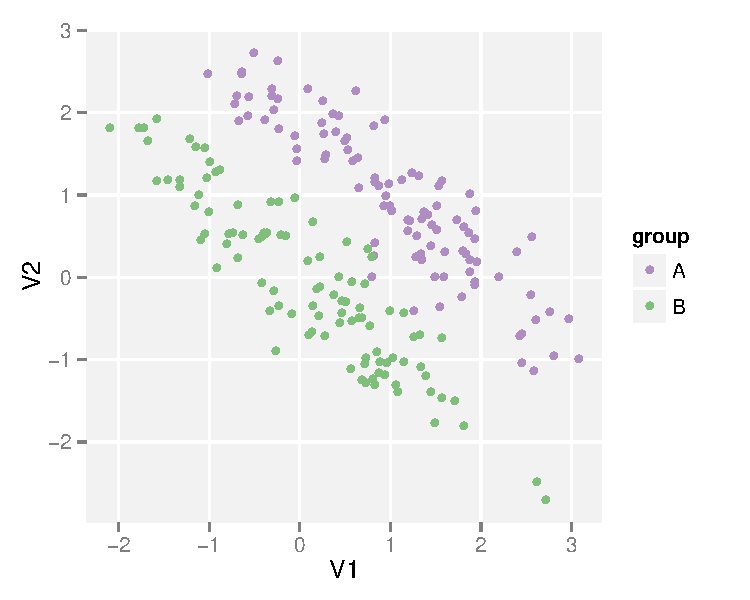
\includegraphics[width=2in]{manova-example}
    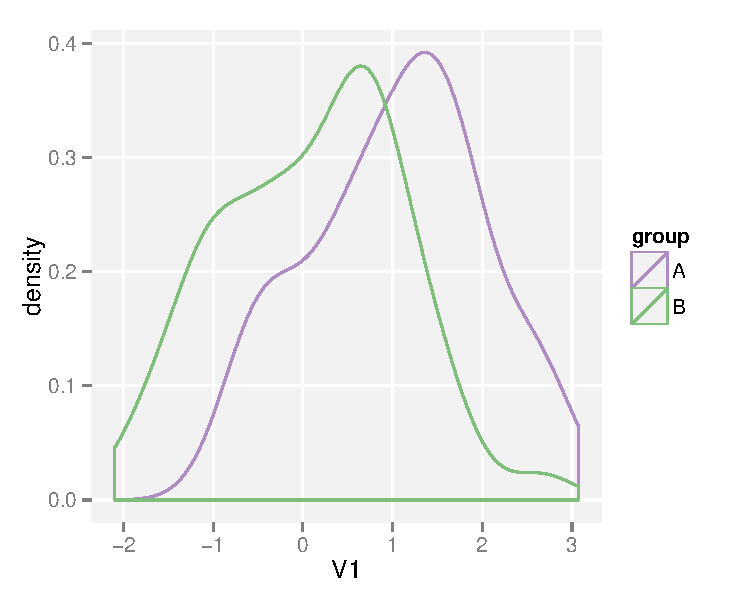
\includegraphics[width=2in]{manova-example-m1}
    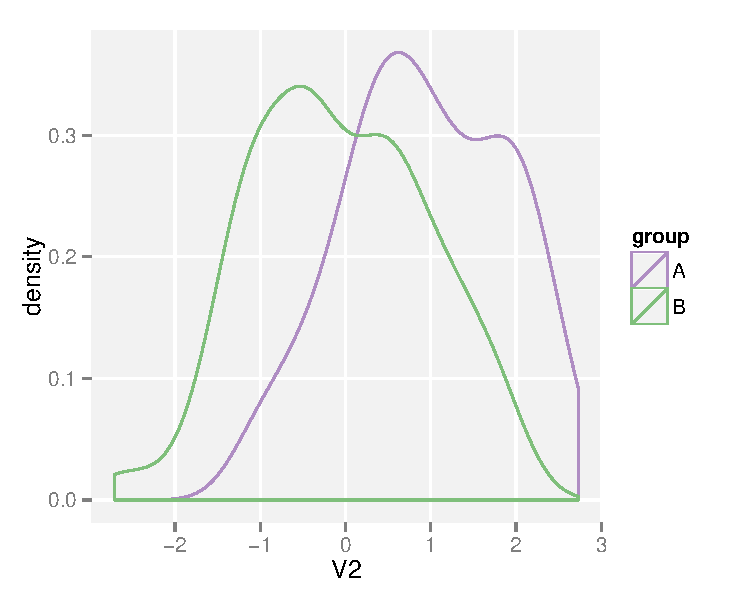
\includegraphics[width=2in]{manova-example-m2}
  \caption{Example where {\sc manova} would detect a difference between the groups, but two {\sc anova}s would not.  Groups are distinct in 2D (left), but overlap on both margins (right).}
  \label{fig:manova-ex}
\end{figure}

This case study explores adding {\sc manova} model information to the raw data. We  investigate a simple {\sc manova} with a single categorical explanatory variable, and discuss how we might extend the ideas to the general multivariate linear model. In this simple case, we model each group using a multivariate normal with the same variance-covariance matrix. To summarize this model we  display a 95\% confidence region around each of the means.

Figure~\ref{fig:manova-wine} shows the result of this approach applied to wine. As the variables are not directly comparable, they have been standardized to range $[0, 1]$.

%This level was proposed by \citet{velleman:1981} as a useful heuristic for comparing two means, and it works reasonably well regardless of whether or not the two distributions have the same variance: if the two regions do not overlap then we can be fairly confident that the means are significantly different at the 5\% level.

% Generating the points on the surface of the confidence region is straightforward.  First, we draw points from a $d$-dimensional standard multivariate normal, then project these onto the surface of a sphere by normalizing each row to distance 1.  Next, we skew this sphere to match the desired variance-covariance matrix, blow it up to give the appropriate $cl$-level confidence ellipsoid, and translate it by the group mean.  This generates a $p$-dimensional ellipsoid, which in 2D projections will look like a filled ellipse.

\begin{figure}[htbp]
  \centering
  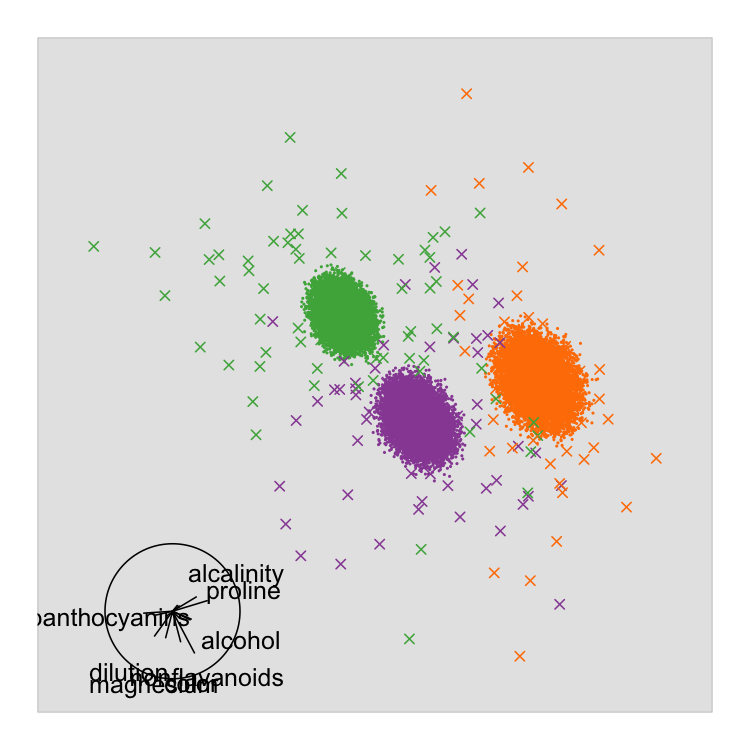
\includegraphics[width=2.5in]{manova-1}
  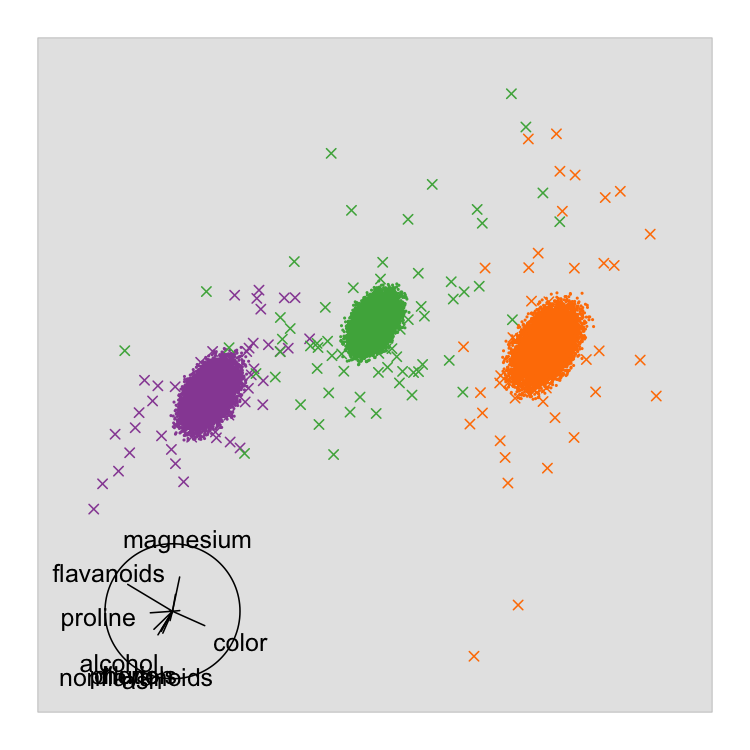
\includegraphics[width=2.5in]{manova-2}
  \caption{Two projections of the wine data with 95\% confidence regions around the group means.  Large points are data, small points are a sample on the surface of the confidence region.  While the confidence ellipsoids appear close in a few projections (left), in most views we see that the means are distant (right).}
  \label{fig:manova-wine}
\end{figure}

% In most cases {\sc manova} is very not interesting because the null hypothesis, that the group means are equal, is unlikely to be true.  We could make this visualization more exploratory by using group-wise covariances to relax the assumption of equal variances, or by using non-parametric density estimation to relax the assumption of normality.

Extending this idea to deal with multivariate linear models is straightforward, although visualizing the resulting surfaces is difficult.  If the model contains continuous variables, then we  no longer have point predictors of the mean, but instead, continuous functions each surrounded by a confidence region.  We can generate these confidence regions by randomly sampling the predictor space and then generating the confidence region for each sampled point as for {\sc manova}.  Visualization is complicated when we have multiple response and predictor variables as we want to keep them separate, e.g.,\ a linear combination of a predictor and a response variable probably does not make much sense.  A potentially useful tool here is the correlation tour \citep{buja:1996}, a version of the tour which uses separate sets of variables for the x and y axes.

 % If only interested in certain terms of the {\sc manova}, can use population marginal means \citep{searle:1980} to marginal over the variables that are not of interest.  We should also take care to correction for multiple comparisons (e.g.\ Scheffe's, because making all possible linear comparisons).  Correlation tour will be useful for exploring these regions because it can display a linear combination of responses on the $y$-axis, and predictors on the $x$-axis.

\subsection{Case study: Classification models}
\label{sub:classifly}

A classifier is a model with a categorical response.  Typically, the classifier is treated as a black box and the focus is on finding classifiers with high predictive accuracy. For many problems the ability to predict new observations accurately is sufficient, but it is interesting to learn about how the algorithms operate by looking at the boundaries between groups. Understanding the boundaries is important for the underlying real problem because it tells us where the groups differ. Simpler, but equally accurate, classifiers may be built with knowledge gained from visualizing the boundaries, and problems of over-fitting may be intercepted.

Much of what we know of how a classifier works is based on the knowledge of the algorithm.  Each family of classifiers partitions the data space in a different way: {\sc lda} \citep{fisher:1936} divides up the data space with hyperplanes, while trees \citep{breiman:1984} recursively split the space into boxes.  Most classifiers produce connected areas for each group, but there are exceptions, e.g.,\ k-nearest neighbors.  To visualize the model in the data space, we can either display the complete prediction regions or just their boundaries.  These two approaches are shown in Figure~\ref{fig:2d}.

\begin{figure}[htbp]
	\centering
	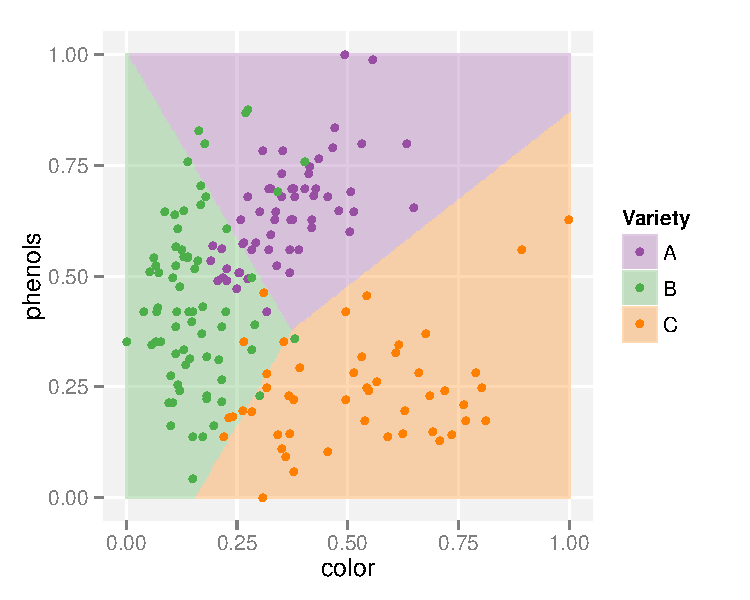
\includegraphics[height=2in]{class-2d-shade.pdf}
	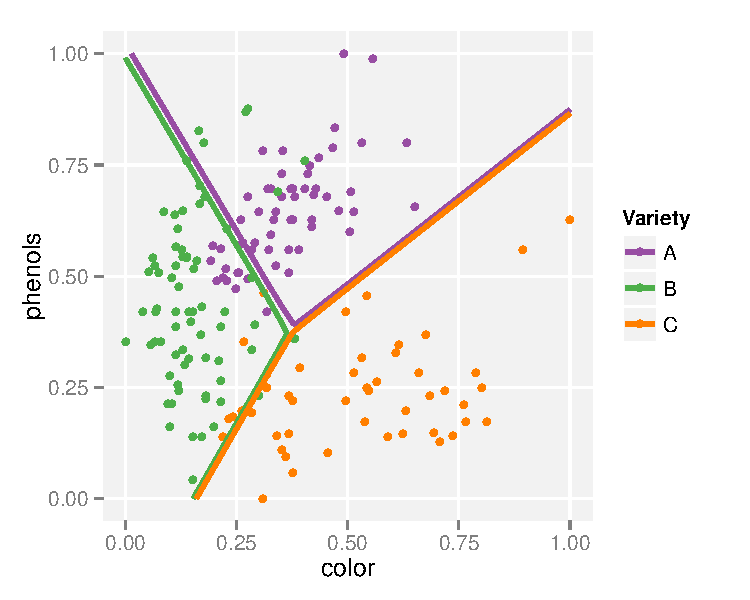
\includegraphics[height=2in]{class-2d-boundary}
	\caption{A 2D {\sc lda} classifier on the wine dataset.  (Left) entire classification region shown and (right) only the boundary between regions.  Data points are shown as large circles.}
	\label{fig:2d}
\end{figure}

Generating the complete prediction region is straightforward: sample many points from data space and classify each one.  Generating only the boundary is more difficult.  We may be able to use a closed form expression if available, but otherwise we can start with the full region and then remove non-boundary points.  To determine if a point is near a boundary, we look at the predicted class probabilities.  If the highest and second highest probabilities are nearly equal, then the classifier is uncertain about the class, so the point must be near a boundary. We call this difference in probabilities the {\em advantage}, and to find the boundary we discard points with values above a tolerance.  The thickness of the resulting boundary is controlled by this cut off, and it should be small enough to give a sharp boundary, but large enough that the set of boundary points is dense.  This is a tricky trade-off.  It may be possible to use adaptive sampling, sampling more densely in regions closer to the boundary, to do better.

If the classification function does not generate posterior probabilities, a $k$-nearest neighbors approach on the grid of predictions can be used. If the neighbors of a point are all the same class, then the point is not on a boundary.  This method can be applied to any classification function, but is slow, $O(n^2)$, because it computes all pairwise distances to find the nearest neighbors.  In practice, this imposes a limit of around 20,000 points.

Figure~\ref{fig:svm-radial3} illustrates the results of a support vector machine \citep{cortes:1995} with radial kernel fitted to three variables from the wine data.  We see the purple region is contained almost completely inside the green region, except where it abuts the orange region. The boundaries and regions are straightforward to understand because our brains are adept at 3D modeling. The video at \url{https://vimeo.com/125405961} explores the boundaries in another way, by brushing along the advantage variable. This shows that the boundaries are equally sharp between the different groups.

As we move beyond 3D it gets harder to see what is going on, but if we persevere we can find informative views. Figure~\ref{fig:svm-poly5} shows three informative views of a polynomial kernel with five variables.  It looks like the boundary is relatively flat (linear) between the orange and purple groups, but quadratic around the green group.  This is easier to see interactively, as at \url{https://vimeo.com/125405962}.

\begin{figure}[htbp]
  \centering
    \includegraphics[width=2in]{3-classifly/svm-radial-2}
    \includegraphics[width=2in]{3-classifly/svm-radial-1}
    \includegraphics[width=2in]{3-classifly/svm-radial-3}
    \includegraphics[width=2in]{3-classifly/svm-radial-4}
    \includegraphics[width=2in]{3-classifly/svm-radial-5}
    \includegraphics[width=2in]{3-classifly/svm-radial-6}
  \caption{Views of a 3D radial {\sc svm} classifier on the wine data using the variables color, phenols, and flavonoids. The same projection is shown with selected subsets of all of the features. (Top left) Data only, (Top middle) Boundary points between the three groups, revealing the highly non-linear decision regions, (Top right) Prediction region for the purple group shown illustrating the way that the classifier wraps the boundary tightly around this group, (Bottom left) Prediction region for the orange group carves out a slice of the cube, (Bottom middle) Prediction region for the green group is basically the rest of the cube, (Bottom right) all three prediction regions colored showing how the cube is carved into the three prediction regions.  Animated version available at \url{https://vimeo.com/125405961}.}
  \label{fig:svm-radial3}
\end{figure}

\begin{figure}[htbp]
  \centering
    \includegraphics[width=1.5in]{svm-poly1}
    \includegraphics[width=1.5in]{svm-poly2}
    \includegraphics[width=1.5in]{svm-poly3}
    \includegraphics[width=1.5in]{svm-poly4}
  \caption{Views of a 5d {\sc svm} with polynomial kernel on the wine data using the variables color, phenols, flavonoids, proline and dilution.  It's possible to see that the boundaries are largely linear, with a ``bubble'' of green pushing into the orange and purple.  A video presentation of this tour is available at \url{https://vimeo.com/125405962}.}
  \label{fig:svm-poly5}
\end{figure}

These ideas are implemented in the R package {\tt classifly} \citep{classifly}, which can visualize classifiers generated by {\sc lda} and {\sc qda} \citep{mass}, {\sc svm} \citep{e1071}, neural networks \citep{mass}, trees \citep{rpart}, random forests \citep{randomForest} and logistic regression; and it can easily to be extended to deal with other classifiers.  More specific visualizations may also be useful for each of these families of models: Section~\ref{sec:nnet} discusses neural networks; \citet{cook:2007}, support vector machines; and {\sc klimt} provides many tools for visualizing trees \citep{urbanek:2002,urbanek:2002a,urbanek:2003}.

\subsection{Case study: Hierarchical clustering}
\label{sub:hierarchical}

Agglomerative hierarchical clustering methods \citep{hartigan:1975a} build up clusters point by point, iteratively joining the two closest points or clusters. The most common visualization of a hierarchical clustering is a dendrogram, a d-in-ms display. There are also a number of other methods of this type: icicles \citep{kruskal:1983}, silhouettes \citep{trauwaert:1989} and clustergrams \citep{schonlau:2002}. Figure~\ref{fig:wine-dendro} shows two dendrograms produced by clustering the wine dataset with Wards linkage and single linkage. These dendrograms are not very informative. For the Wards clustering we can see that there are three major clusters, and for single linkage the clusters seem to grow mainly by adding a single point to an existing cluster. We cannot see what the clusters have in common, or what variables are important for the clustering.

% This requires a distance metric, and a method for calculating the distance between two clusters (linkage).  There are a number of common methods:  use the closest distance (simple linkage), the largest distance (complete linkage), the average distance ({\sc upgma}), or the distance between cluster centroids (Ward's).  Each of these methods finds clusters of somewhat different shapes: single linkage forms long skinny clusters, average linkage forms more spherical clusters.

\begin{figure}[htbp]
  \centering
    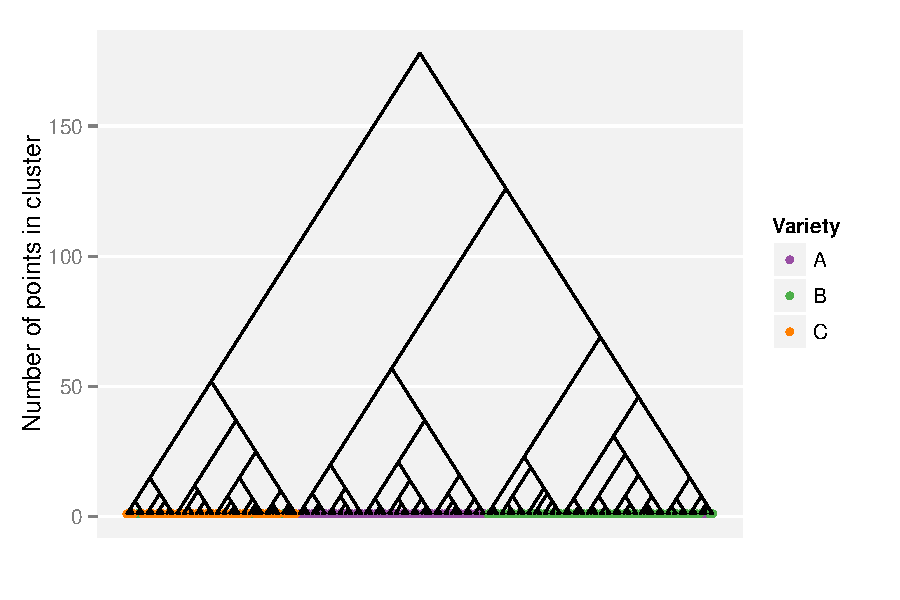
\includegraphics[width=0.45\textwidth]{wine-ward}
    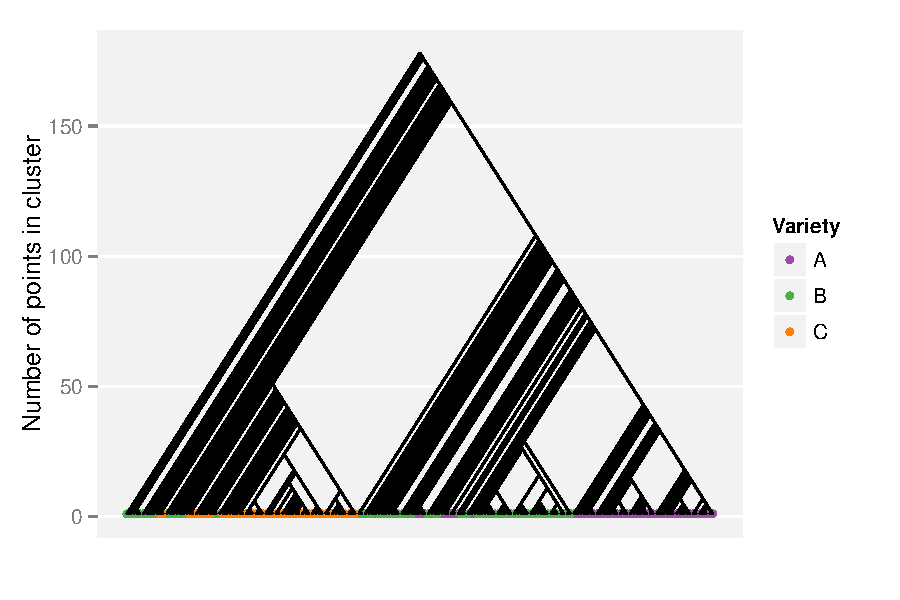
\includegraphics[width=0.45\textwidth]{wine-single}
  \caption{Dendrograms from a hierarchical clustering performed on the wine dataset.  (Left) Wards linkage and (right) single linkage.  Points colored by wine variety.  Wards linkage finds three clusters of roughly equal size, which correspond fairly closely to three varieties of wine.  Single linkage creates many clusters by adding a single point, producing the dark diagonal stripes. }
  \label{fig:wine-dendro}
\end{figure}

To do better we need to display the model in data space.  \citet{buja:1996} draws inspiration from the dendrogram and suggests an interesting idea: connect the observations in the data space according to their hierarchy in the clustering.  For intermediate nodes in the hierarchy, representing clusters containing more than one point, we supplement the data with extra points located at the cluster centroid.   An extension would be to connect clusters in the same way as inter-cluster distances are calculated, i.e.,\ connect closest points for single linkage, most distant for complete, and centroids for Wards.  Another approach is described in \citet{kim:2000} which uses {\sc mds} for dimension reduction, and overlays the minimum spanning tree.

Figure~\ref{fig:wine-ggobi} displays some views of the wine dataset supplemented with a hierarchical clustering with Wards linkage.  It is easy to see the three groups and the hierarchical links in the tour, as shown at \url{http://www.vimeo.com/768329}.

\begin{figure}[htbp]
  \centering
    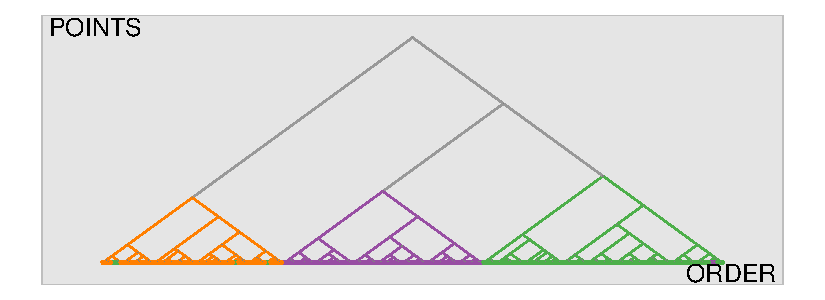
\includegraphics[width=5.2in]{wine-hcward-1}
    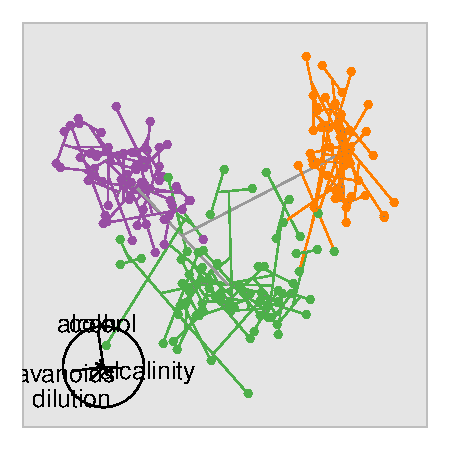
\includegraphics[width=2.5in]{wine-hcward-2}%
    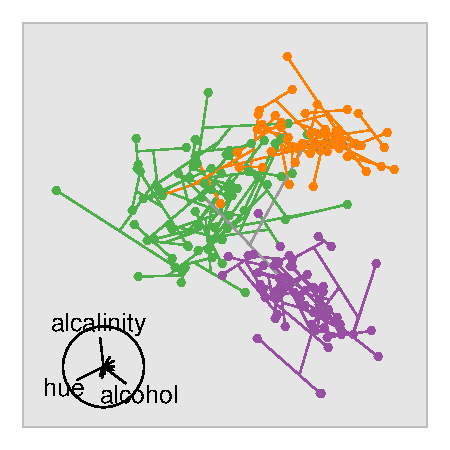
\includegraphics[width=2.5in]{wine-hcward-3}
  \caption{(Top) A dendrogram with points colored by variety and edges colored by majority membership. (Bottom) Two informative projections of the data space show that the varieties are arranged in a rough {\sf U} shape, with a little overlap, and some of the outlying orange points have been clustered with the green points.}
  \label{fig:wine-ggobi}
\end{figure}

An implementation of these ideas is available in the {\tt clusterfly} package \citep{clusterfly}.

\section{Collections are more informative than singletons}
\label{sec:collections}

So far we have looked at visualizing a single model in the data space, but collections of models arise in many ways, and in most cases most of the models are ignored and we only look at the best model. This is perilous as we may miss alternative models that explain the data almost as well as the best model, and suggest substantially different explanations for the phenomenon of interest. A few of the ways that collections are produced include:

\begin{itemize} \itemsep 0in
  \item From exploring the space of all possible models.  For a given model family, we can generate all possible model forms, e.g., for a linear model, we can generate all possible linear models with main effects.  As this  often produces too many models to possibly fit or compare, we typically employ some model selection algorithm to explore the space of ``best'' models, and only the best, or maybe the two or three best models are examined.

  \item During the the process of data analysis.  When analyzing a data set, we may create and discard many models in an attempt to reveal the salient features of the data.  It may be useful see all of these models simultaneously.

  \item While trying to find a global optima. When model fitting is not guaranteed to converge to a global optimum, we may have a collection generated from multiple random starts.  This is useful for multidimensional scaling, neural networks, k-means clustering, and self organizing maps.  Typically, only the model with the highest criterion value is examined.

  % \item May have been created explicitly to model prediction, or to more accurately account for the degrees of freedom used up by model selection.  i.e. in model averaging, we combine multiple models weighted according to their predictive ability.

  \item By varying model settings.  If a model has some tuning parameters, we can systematically alter them and observe the result, e.g.,\ the penalty parameter in lasso, or the degrees of freedom in a smoothing term.  Often, cross-validation is used to select a single optimal model.

  \item By fitting the same model to different datasets.  These datasets might be groups within a larger dataset (perhaps a prequel to fitting a mixed effects model), or might have been generated by leaving-one-out, cross validation, bootstrapping, permuting, simulating, as part of a sensitivity analysis or by adding random noise to the response \citep{luo:2006}.  Typically, these multiple models are collapsed into a small set of summary statistics.

  \item As an intrinsic part of the model.  Certain model families use ensembles of simple sub-models: neural networks (ensembles of logistic models), random forests (ensembles of trees), bagging, and boosting. Typically, we just look at the overall model, and ignore how each part contributes to the whole.

  \item By treating each iteration as a model.  If we are interested in exploring the process of model fitting, and the algorithm is iterative, we might treat each iteration as a separate model.  This gives a unique ordering to the models and is described in depth in Section~\ref{sec:iteration}.  Typically, we only look at the last iteration.

\end{itemize}

What can we do if we want to visualize such a collection? One approach is to visualize all models simultaneously. This is the strategy of trace plots \citep{urbanek:2005}, which show hundreds of tree models simultaneously. This makes it possible to see the space of models, showing both the common and the unusual. However, in most cases we are not able to view more than a couple of models simultaneously because they will overlap and obscure one another.

To work around this problem, we need to be able to fluidly explore smaller sets of interesting models. We can do this by calculating descriptive statistics on multiple levels, then using linked brushing to connect these statistics to one another and to displays of the model. These ideas grow out of exploratory model analysis \citep{unwin:2003aa,urbanek:2004} and draw on fundamental ideas of descriptive statistics \citep{bickel:1975a,bickel:1975b}. Here we focus on displays of model space, with the assumption that these displays are linked to additional m-in-ds displays to help us tune our descriptive statistics to match the model features of interest.

The first level of descriptive statistics summarizes model quality: a trade-off between complexity and fit. Model complexity is often summarized by degrees of freedom, but there may be more informative measures for specific model families, e.g.,\ the number of hidden nodes in a neural network. The fit can be summarized by the likelihood at the parameter estimates of models fit using the {\sc ml} algorithm, or by some measure of predictive ability. These statistics help us explore overall model quality and the tradeoff between quality and complexity, but do not give any information about how the models differ, how the fit of a given observation varies between models, or what exactly the parameter estimates are.

To explore these aspects of the model, we need descriptive statistics at other levels. A good example of a statistical procedure with built in summary statistics at additional levels is the random forest \citep{breiman:2001}, an ensemble method which uses many simple trees fit to random subsets of the variables and observations. As well as the model-level summaries described above, random forests provide tree-level, variable-level and observation-level descriptive statistics:

\begin{itemize}
  \item Tree-level.  Each tree in the ensemble has its own test and training data sets and so can compute an unbiased estimate of classification error.  Inspecting these errors allows us to find trees that perform particularly well or poorly.  Looking at many good trees in the data space, allows us to see commonalities (suggesting important variables) and differences (suggesting correlations between variables).

  \item Variable-level.  Each variable is ranked by the drop in model performance when that variable is randomly permuted. This is a summary of a tree-variable statistic, which computes variable importance for each tree.

  \item Observation-level.  For each observation we have the distribution of predictions across all trees.  This can show which observations are easy (or hard) to classify, and which classes are most often confused.

\end{itemize}

For other models, we  need to develop and calculate our own descriptive statistics. Often there exists a large body of literature with suggestions for statistics. Another approach is to calculate a familiar summary statistic over an unfamiliar population. For example, we could calculate an observation-level summary by averaging the observation's residual over all the models. If models in the collection have common parameters, we might create parameter-level summaries of the distribution of the estimates over the models. The important thing is to generate descriptive statistics at multiple levels, in order to gain maximum insight into the models.

Once we have computed the summary statistics, we need to explore them. Static plots are helpful, but make it difficult to link between summaries at different levels. For example, we might want to see how the model-estimate summaries differ between the best and second best models. Linked brushing is particularly useful here. We can have one plot of model-level statistics and one of model-estimate-level statistics and use brushing to link between them. This idea is described in more detail in the case study.

The {\sc raft} tool \citep{raft} for visualizing random forests provides a good set of static graphics, but provides no way to link between the plots, and no m-in-ds visualizations. This is a problem: if we found a single tree that did a particularly good job, we would like to see how it divides up the data space. Without linked graphics it is difficult to see exactly what is going on within a random forest, and to see how they compare to other models.  The following case study shows how summary statistics and linked graphics can be used to gain insight into ensembles of linear models.

\subsection{Case study: Linear models}
\label{sec:linear-models}

In this case study we  explore a collection of linear models containing a large subset of all possible main effects models. Let us assume that we have $m$ models describing a data set with $n$ observations and $p$ variables. If all possible main effects models are fit, there are $m = 2^p - 1$ models in the collection. We  explore summary statistics on five levels:

\begin{itemize} \itemsep 0in
  \item Model level: model fit statistics.  $m$ observations.
  \item Model-estimate level: coefficient estimates on various scales.  $m \times p$ observations.
  \item Estimate level: summary of estimates over the models.  $p$ observations.
  \item Model-observation level: residuals and influence measures.  $m \times n$ observations.
  \item Observation level: the original data, plus summaries of residual behavior. $n$ observations.
\end{itemize}

\noindent The relationship between these different levels is shown schematically in Figure~\ref{fig:summaries}.

In this case study, we  use a data set on 2006 house prices in New Haven, Connecticut \citep{emerson}. We are interested in predicting price based on characteristics of the house. There are 18,221 observations and 6 predictor variables, resulting in a collection of 63 ($2^6 - 1$) models. The predictors include size of the living area ({\tt livingArea}), size of the house ({\tt size}), zone ({\tt zoneRM}), presence of air conditioning ({\tt acType}), number of bedrooms ({\tt bedrms}) and bathrooms ({\tt bathrooms}). We  focus on the  model and model-estimate level summaries. The remainder are discussed more fully in \citet{wickham:2007h}.
\hh{XXX what is the remainder? Could you be more specific?}

\begin{figure}[htbp]
  \centering
    \includegraphics[width=4in]{summaries}
  \caption{Relationship between five levels of summary statistics for a collection of linear models. Arrows indicate one-to-many relationships, e.g.,\ for each model-level summary, there are many model-observation and model-estimate statistics.}
  \label{fig:summaries}
\end{figure}

\paragraph{Model summaries} Figure~\ref{fig:model} shows model-level summary statistics: model complexity and model fit. We use one measurement of model complexity (degrees of freedom) and five standardized measurements of model fit: log-likelihood, AIC, BIC, $R^2$ and adjusted $R^2$. The relationship between complexity and fit is very similar across measures, with improvement in model quality decelerating as model complexity increases. The improvement plateaus after five degrees of freedom (three variables), but small improvements can still be gained by including two more variables.

\begin{figure}[htbp]
	\centering
  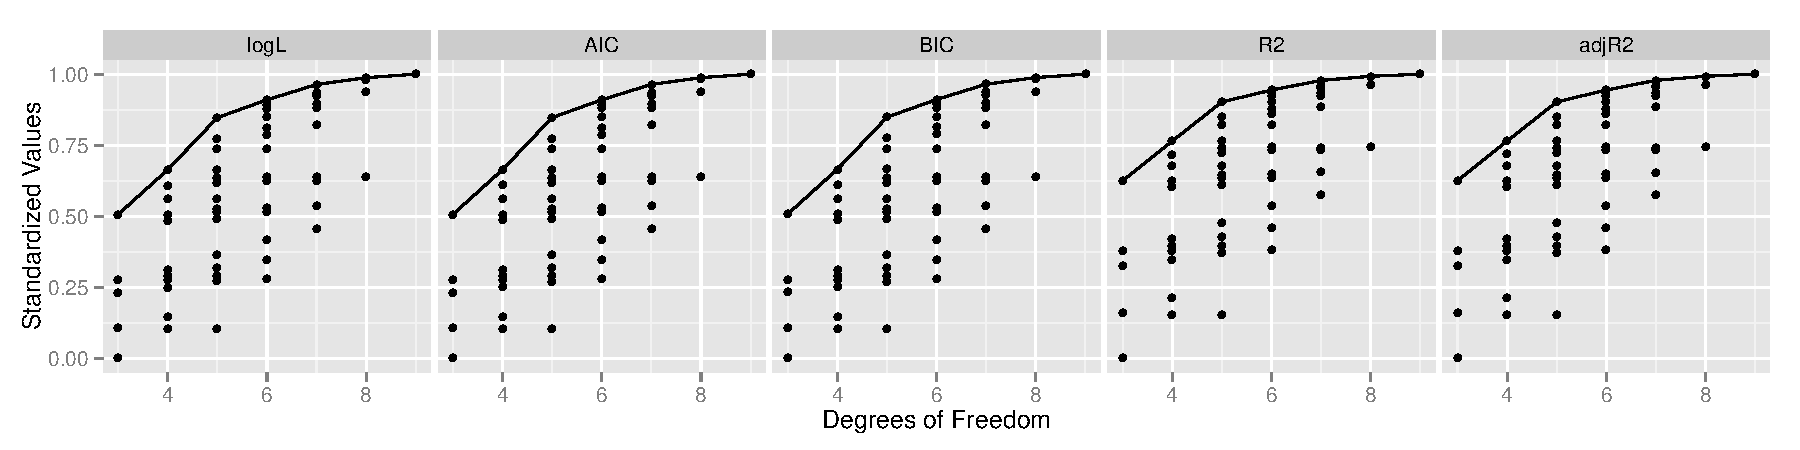
\includegraphics[width=\linewidth]{houses-coef-models.pdf}
	\caption{Model summary statistics, each scaled to $[0,1]$ to aid comparison.  A line connects the best models for each degree of freedom.  The intercept only model is not displayed.  Degrees of freedom include calculation of intercept and variance.  These summary statistics suggest that a either five df/three variable or a seven df/five variable model are good tradeoffs between complexity and performance.}
	\label{fig:model}
\end{figure}

\paragraph{Model-estimate summaries} Each model contains between $1$ and $p$ variables, and for each variable in each model we calculate:

\begin{itemize} \itemsep 0in
	\item The raw estimate, useful when all predictors are on the same scale.

	\item The standardized estimate, generated from models fit to standardized predictors. These are useful as measures of relationship strength for each variable because they can be interpreted as the change in response when the predictor changes by one standard deviation if all other variables are held constant.

	\item The $t$-statistic and absolute $t$-value, allowing us to assess the significance and direction of the relationship between the response and predictor.
\end{itemize}

We can use this graphic to explore the importance of the predictors. There are two interesting examples of this in Figure~\ref{fig:coef}. First, the standardized estimates of {\tt livingArea} are very similarly positive and large across all models, which suggests that it is the most important variable in predicting housing price. (A value of 0 indicates models in which the variable was not included.) Another interesting phenomenon is the behavior of the estimates for the {\tt bedrms} variable. For some of the models the estimates are negative, suggesting that houses with more bedrooms have lower prices! For other models the relationship is what we would expect, positive coefficients and a positive relationship with price.

\begin{figure}[htbp]
	\centering
	\includegraphics[width=0.8\textwidth]{houses-stdcoefs}
	\caption{Standardized coefficients by variable, so we can judge relative strength on a common scale. The {\tt livingArea}, {\tt size}, {\tt zoneRS}, and {\tt bathrm} variables always have positive coefficients suggesting positive association with price. The {\tt bdrms} variable has mixed coefficients, some positive and some negative.}
	\label{fig:coef}
\end{figure}

Figure~\ref{fig:coef-upag} uses linked brushing to highlight these models and to examine the fit more closely. We have two plots visible simultaneously, and link the same models between them. The plots on the left side are parallel coordinate plots of the standardized estimates by variable, and plots on the right side show the $R^2$ by degrees of freedom of the models. In the top row, models with positive coefficients for bedrooms are highlighted in red. These models are surprisingly bad! They have the smallest $R^2$ values for their relative degrees of freedom. Looking at the plot of estimates shows that these models are all missing the living area variable. Models with negative coefficients for bedrooms are highlighted in the bottom row of plots. These are all good models, with high $R^2$, and they are also models where living area is included. This suggests collinearity between living area and bedrooms. Exploring these pairs of plots generally helps us to analyze the covariance structure between predictors and the effect on the response.

\begin{figure}[htbp]
	\centering
  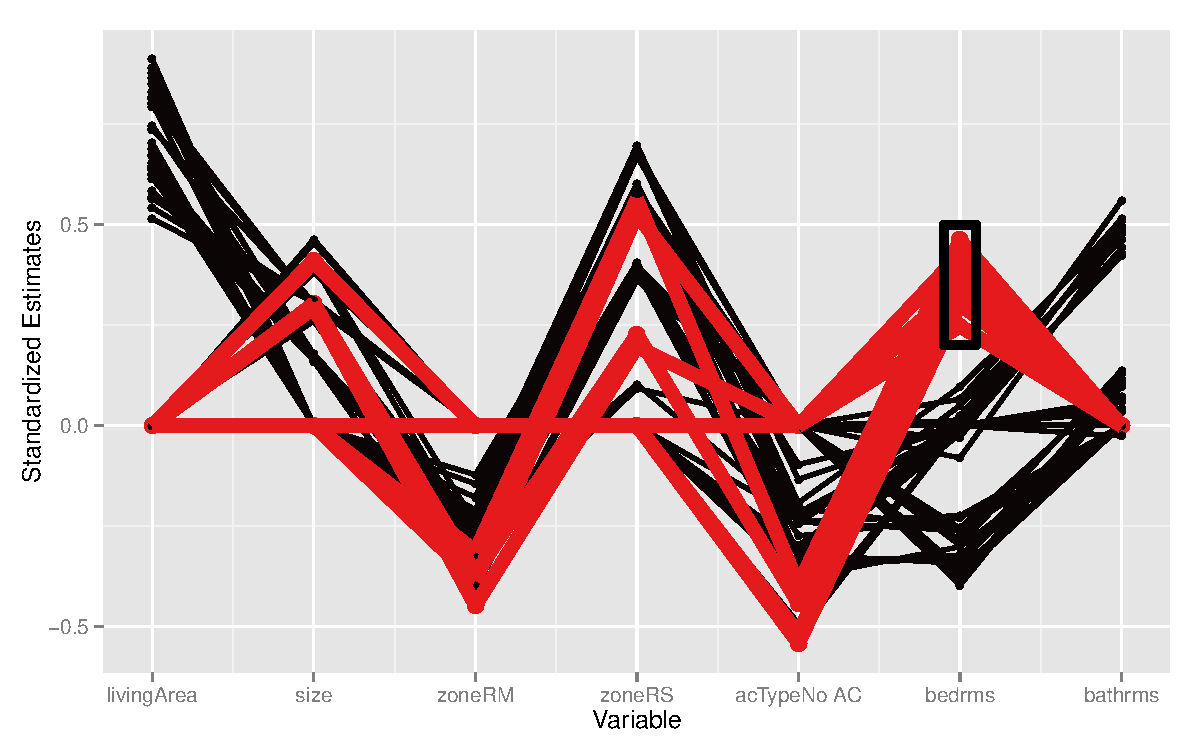
\includegraphics[width=0.5\textwidth]{houses-brushing1}
  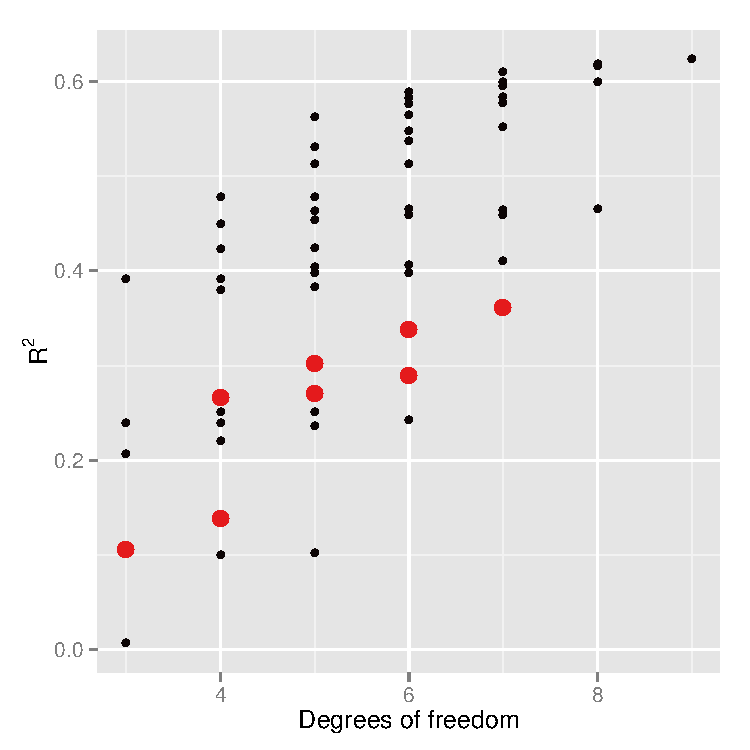
\includegraphics[width=0.31\textwidth]{houses-brushing2}

  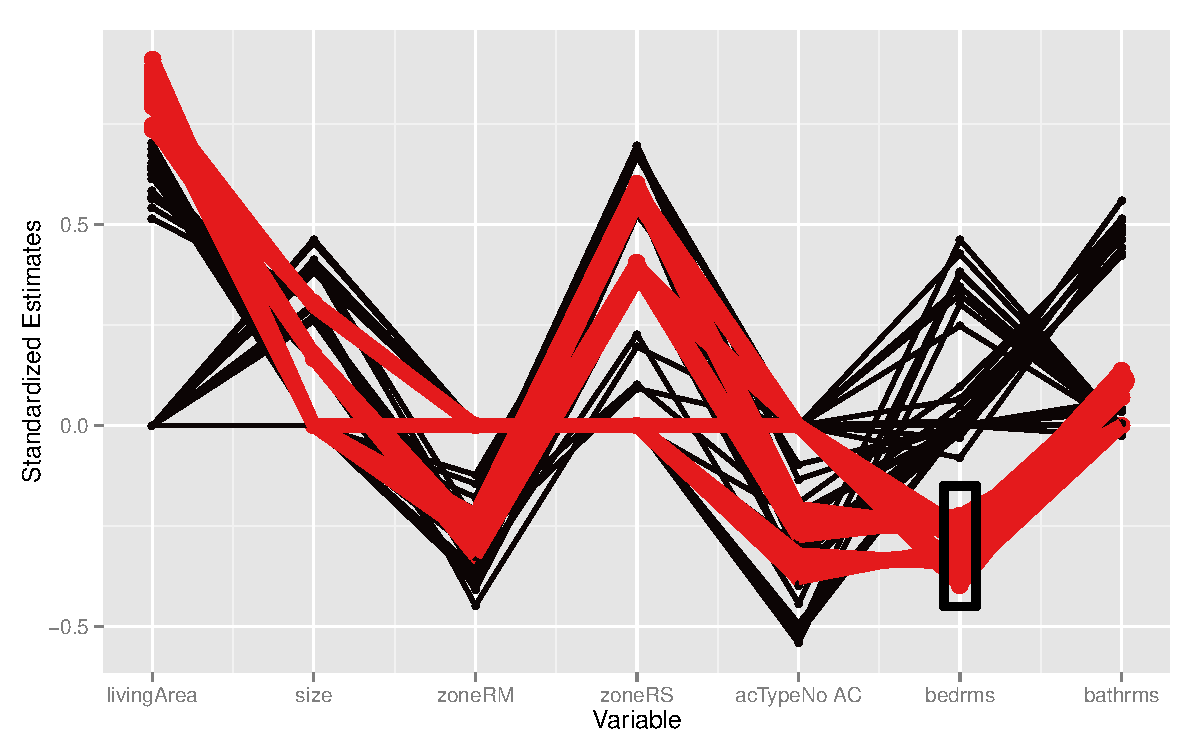
\includegraphics[width=0.5\textwidth]{houses-brushing3}
  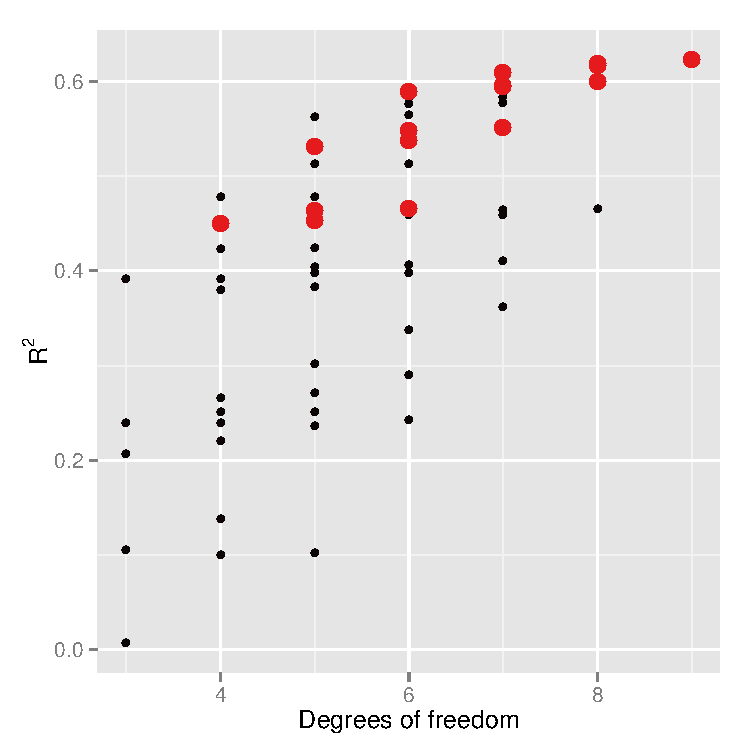
\includegraphics[width=0.31\textwidth]{houses-brushing4}

	\caption{(Left) Parallel coordinates plot of standardized estimates vs variable.(Right) Scatterplot of $R^2$ vs degrees of freedom. Subsets of models are selected (red) based on their estimates for {\tt bedrms}. (Top) Models with positive estimates have low $R^2$ values and do not include {\tt livingArea}. (Bottom) Models that have negative estimates for {\tt bedrms} have high $R^2$ and also high coefficients for livingArea. This would suggest  collinearity between these two variables.}
	\label{fig:coef-upag}
\end{figure}

%Figure~\ref{fig:coef-ggobi} shows another way to use these linked plots, by highlighting the two best models and then inspecting their standardized coefficients.  We can see that the best and second best models differ on inclusion of the examination variable.

%\begin{figure}[htbp]
%	\centering
%  \includegraphics[width=0.45\textwidth]{coef-models}
%  \includegraphics[width=0.45\textwidth]{coef-coefs}
%
%	\caption{(Left) Scatterplot of $R^2$ vs degrees of freedom.   (Right) Parallel coordinates plot of standardized coefficient vs variable.   The two best models have been highlighted in red in both plots.}
%	\label{fig:coef-ggobi}
%\end{figure}

These ideas are implemented in the {\tt meifly} package ({\bf m}odels {\bf e}xplored {\bf i}nteractively) \citep{meifly} which uses R to fit the models and calculate the summary statistics, and ggplot2 and GGobi to display them.

\section{Do not just look at the final result; explore how the algorithm works}
\label{sec:iteration}

Whenever we can gain insight into the process of model fitting, we should. Observing iterations helps us understand how the algorithm works and can reveal potential pitfalls. Developing suitable visualizations forces us to think deeply about exactly what the algorithm does and can suggest possible avenues for improvement. For some algorithms, it may be possible to intervene, contributing a more global perspective to help the algorithm escape local maxima.

Many statistical algorithms are inherently iterative: {\sc irls} in the generalized linear model, the Newton-Raphson method in maximum likelihood, the {\sc em} algorithm, multidimensional scaling, and k-means clustering.  Some of these methods are guaranteed to converge to the global optimum (e.g., {\sc irls}, {\sc em}), but most are not.  We can think of each iteration as its own model, and we want to explore the changes over time.  Many of the messages of Section~\ref{sec:collections} also apply here: we should look at each step, not just the last one; we should try and display all models on a single plot where possible; and if not, we should develop good summary statistics.  The specific feature of collections generated by iteration is that there is a unique ordering of the models.

This ordering suggests two approaches to visualization: ordering in space, to make time series plots, and ordering in time, to make movies.  The time series plot displays time on the $x$-axis and some summary statistic on the $y$-axis, and shows at a glance the progress of a single parameter.  This only works for a small number of numeric summaries, so for more complicated summaries we can make a movie.  A movie strings together many static plots, each of which captures the state of the model at a single point in time.  The {\tt animation} package \citep{animation} is a rich source of animations in R, but only provides one animation that displays the progress of an algorithm, k-means clustering.

To capture the data we need for these plots, we can either stream data updates, replacing the values from the previous iteration; or store all iterations for later exploration.  Streaming updates allows us to intervene in the algorithm and observe the effect of our changes, while storing everything allows us to later run time forwards and backwards.  A particularly nice example of intervening in the progress of an algorithm is {\tt ggvis} \citep{buja:2008}, an interactive tool for multidimensional scaling that allows you to manually drag points out of local optima.

Being able to extract this data is dependent on the implementation of the algorithm.  At a minimum we either need a hook into the algorithm which calls a function every $n$ iterations; or we need to be able to run the algorithm for a fixed number of steps, and to be able to start the fitting process from the results of a previous run.  This is not always straightforward as many algorithms also have time-varying parameters that must be captured and recreated. Typically, extracting and saving this data  considerably slows the algorithm, often by an order of magnitude.

The following two case studies illustrate some of these ideas.  The first case study, on projection pursuit, visualizes the use of simulated annealing to find interesting projections of the data.  The second case study explores the fitting process of self organizing maps, as implemented by the {\tt kohonen} package.

\subsection{Case study: Projection pursuit and simulated annealing}
\label{sub:guided}

The guided tour \citep{cook:1995} is a combination of the grand tour and projection pursuit.  Instead of randomly picking new projections, as in the grand tour, the guided tour only picks new projections that are more interesting, by optimizing an index of interestingness with simulated annealing \citep{kirkpatrick:1983}.  This case study investigates how we can gain insight into the path that the simulated annealing takes. The indices we use in this example come from the graphic theoretic scagnostics of \citet{wilkinson:2005} and are implemented in the {\tt scagnostics} package \citep{scagnostics}.

Figure~\ref{fig:pp-timeseries} shows a time series of the scagnostic index being optimized, clumpiness, which takes high values when the data is grouped into distinct clumps.   We can see that the paths are not monotone: there is a stochastic component to simulated annealing which helps it avoid local optima.  Each of the points on the plot corresponds to a projection matrix, and it is interesting to see if all the peaks correspond to the same or different projections.  Figure~\ref{fig:pp-peaks} shows the four projections with highest clumpiness.  Visualizing the projection matrices themselves is difficult (each column corresponds to a point on a $p$-dimensional hypersphere) but can be revealing \citep{cook:2006}.

\begin{figure}[htbp]
  \centering
  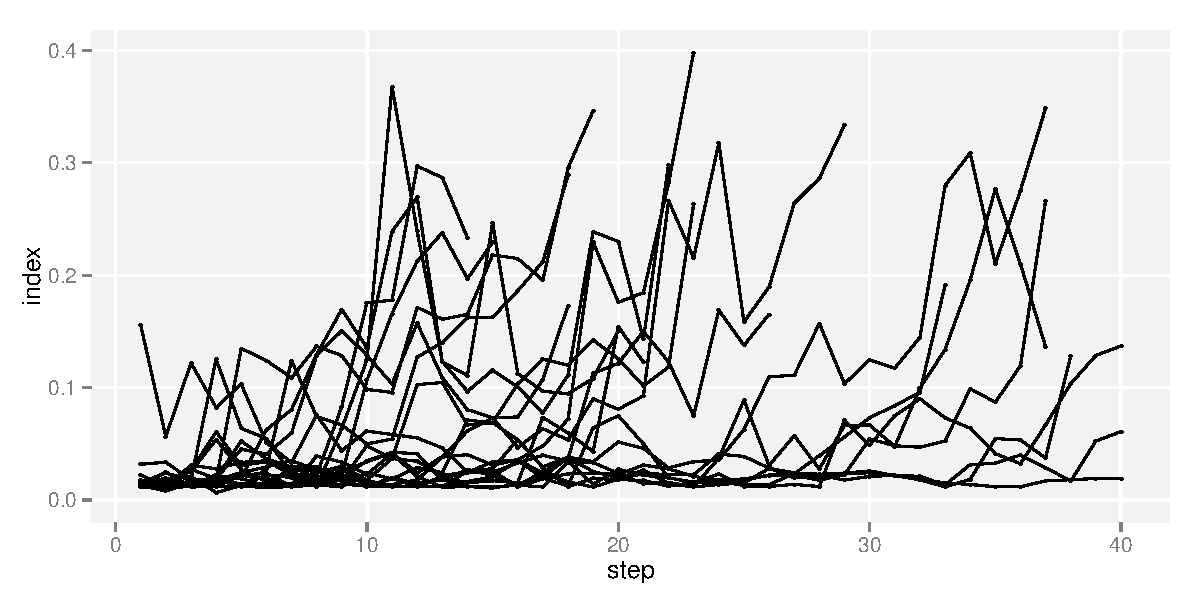
\includegraphics[width=4in]{pp-index-progression}
  \caption{Variation of the clumpy index over time.  Simulated annealing with 20 random starts, run until 40 steps or 400 tries.  Red points indicate the four highest values.}
  \label{fig:pp-timeseries}
\end{figure}

\begin{figure}[htbp]
  \centering
  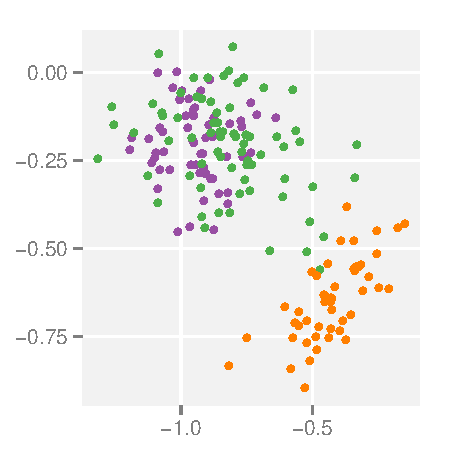
\includegraphics[width=0.24\textwidth]{proj-1}
  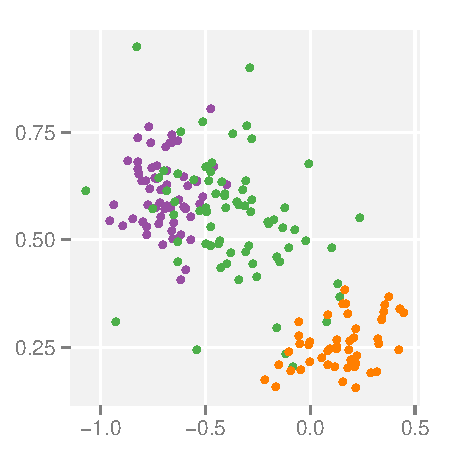
\includegraphics[width=0.24\textwidth]{proj-2}
  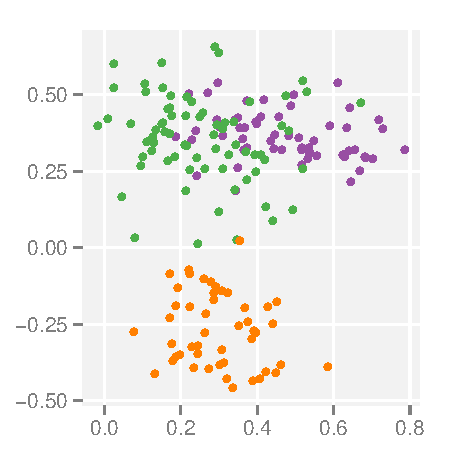
\includegraphics[width=0.24\textwidth]{proj-3}
  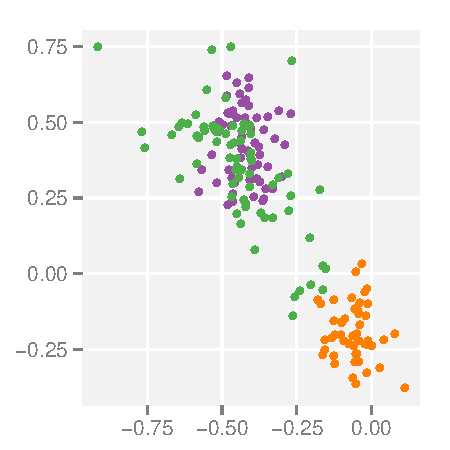
\includegraphics[width=0.24\textwidth]{proj-4}
  \caption{Four projections of the data with highest values of clumpiness, found by the simulated annealing shown in Figure~\ref{fig:pp-timeseries}.  Plots are ordered left to right from highest to lowest.  All these projections have good separation between the orange cluster at the others, but not between the purple and green clusters.  Looking at the top 15 maxima does not find any projections that separate these two groups.  }
  \label{fig:pp-peaks}
\end{figure}

We can also use interaction with this plot to do something rather interesting: restart the simulated annealing from one of the local optima and see if it can do better in that same location.  Figure~\ref{fig:pp-multiple-starts} restarts from a local optima and shows that it is difficult to do better.

\begin{figure}[htbp]
  \centering
  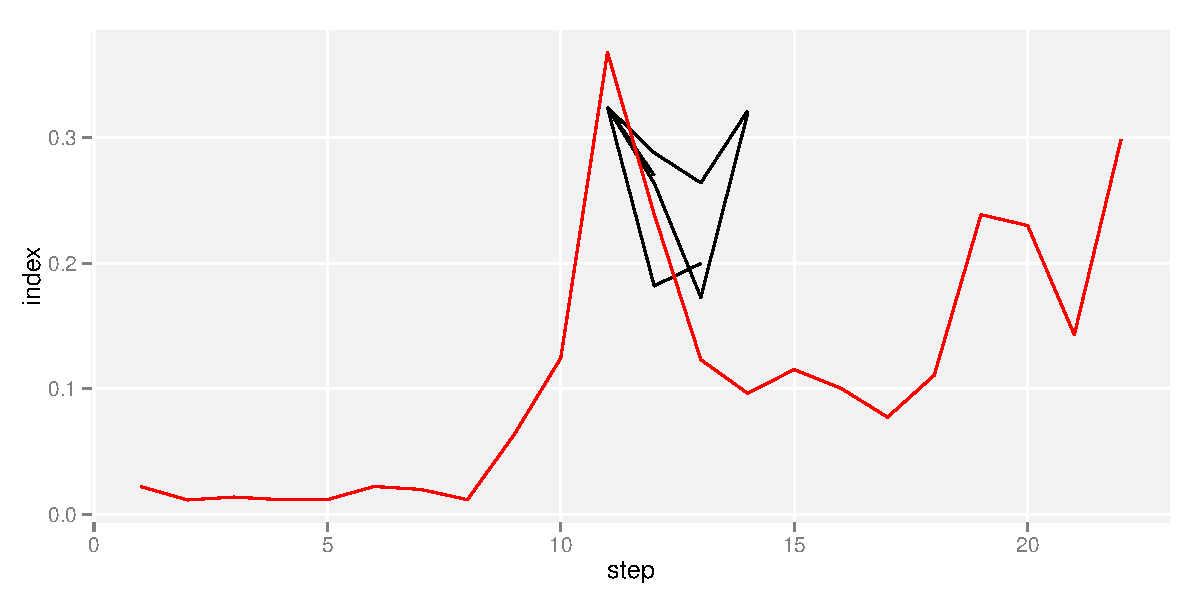
\includegraphics[width=4in]{pp-restart}
  \caption{One of the guided tour runs of Figure~\ref{fig:pp-timeseries} with new guided tours launched from particularly good projections.  Red line shows path of original simulated annealing.}
  \label{fig:pp-multiple-starts}
\end{figure}


\subsection{Case study: self organizing maps}
\label{sub:som}

A self-organizing map ({\sc som}) is a machine learning algorithm which  simultaneously performs clustering and dimension reduction \citep{kohonen:2001}. {\sc som}s are often described as a type of neural network, but they are more easily understood as a type of constrained k-means.   The idea is simple: we are wrapping a net of points into the data cloud. The knots in the net are called nodes, and are constrained by their neighbors.  Each node has a position in the data space (like a cluster centroid), and the model space (a grid coordinate on the net).  In this case study we  look at the self organizing maps implemented in the {\tt kohonen} package \citep{kohonen}.

We first need a method for visualizing the model in the data space.  The majority of {\sc som} displays show the data in the model space, and give little insight into the quality of the model.  An idea for a visualization comes immediately from the net metaphor: we  display the data, the nodes, and the connections between neighboring nodes; a net wrapped through the data.  Figure~\ref{fig:bad-fit} contrasts a typical d-in-ms view (left) with a m-in-ds view (right) for 10 $\times$ 3 node som fit to the wine data. The d-in-ms view shows the positions of each of the nodes of the net using a Coxcomb display. Nodes in the middle of the net have large values on all variables, that is they are close to the (1,1,1,1,1) region in the data space, and nodes on the right and left side have all low values, indicating they are close to (0,0,0,0,0) region  in the data space, assuming the data falls inside a 5D unit cube. In contrast the m-in-ds view shows the nodes relative to the data points, and allows us to see how the model fits to the data, better evaluating the goodness-of-fit. In this one projection the model can be seen to be fairly linear in the 5D space, winding through the three clusters.

\begin{figure}[htb]
  \centering
    \includegraphics[height=2.0in]{wine-som1}
    \includegraphics[height=2.0in]{wine-som2}
  \caption{(Left) A visualization of the model space.  Each node is represented by a Coxcomb plot which represents the position of that node in the data space. (Right) A projection of the model embedded in the data space. }
  \label{fig:bad-fit}
\end{figure}

The algorithm for fitting a {\sc som} is very similar to k-means, but instead of updating a single node at a time, we also update that node's neighbors:

\begin{enumerate}
  \item Randomly initialize nodes to positions in data space.
  \item Iterate through each data point, and assign it to the closest node
  \begin{enumerate}
    \item Update the location of node: $(1 - \alpha) \cdot \textrm{node} + \alpha \cdot \textrm{point}$
    \item Also update the location of all neighboring nodes within distance $r$ on grid
  \end{enumerate}
  \item Decrease $\alpha$ and $r$, and repeat step 2 until stopping condition is met
\end{enumerate}

For the wine dataset, we  fit a 10 $\times$ 3 net: we know the data seems to fall along a 1d path, but  we want to allow for potential structures along another dimension.  To record the progress of the model fit, we  save the following information at each of 100 iterations: the positions of the nodes, the values of $r$ and $\alpha$, and the distance from each point to its corresponding node.

Figure~\ref{fig:som-dist} summarizes the quality of the model fit over time, by plotting the distance between each point and its corresponding node.  Looking at the mean alone is misleading: there is a dramatic drop in mean distance when switching from a radius of three to two.  However, when we look at the complete distribution, we can see that this drop is small compared to the total variation.  We also see a number of outlying points that never get close to a node.  The variation in those lines might also make us wonder if we have stopped the algorithm too soon.

\begin{figure}[htbp]
  \centering
    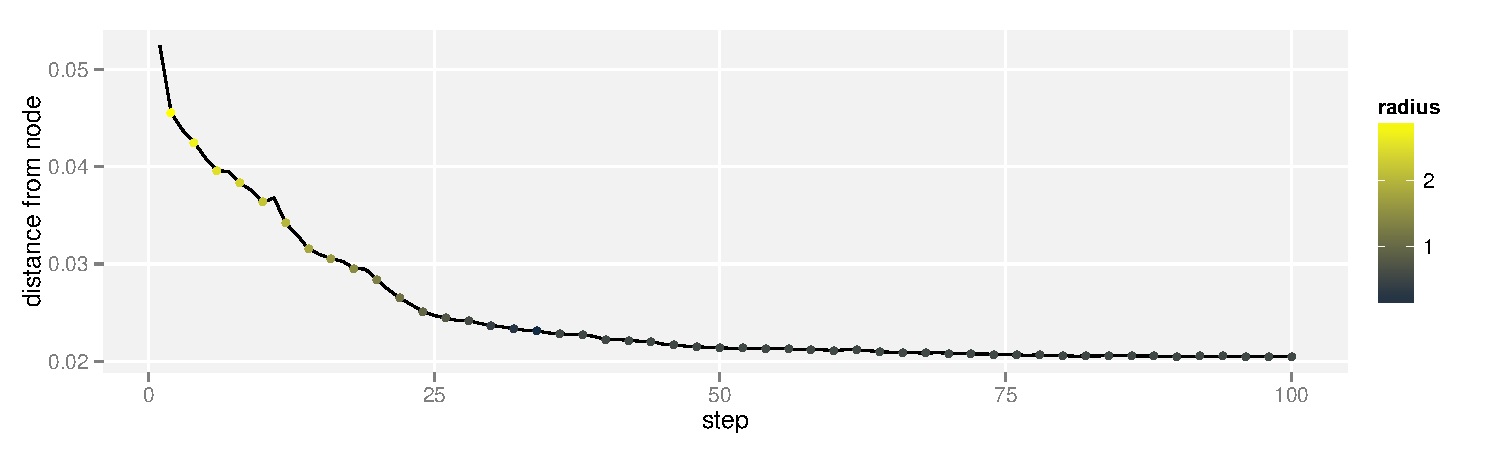
\includegraphics[width=5in]{som-dist-mean}
    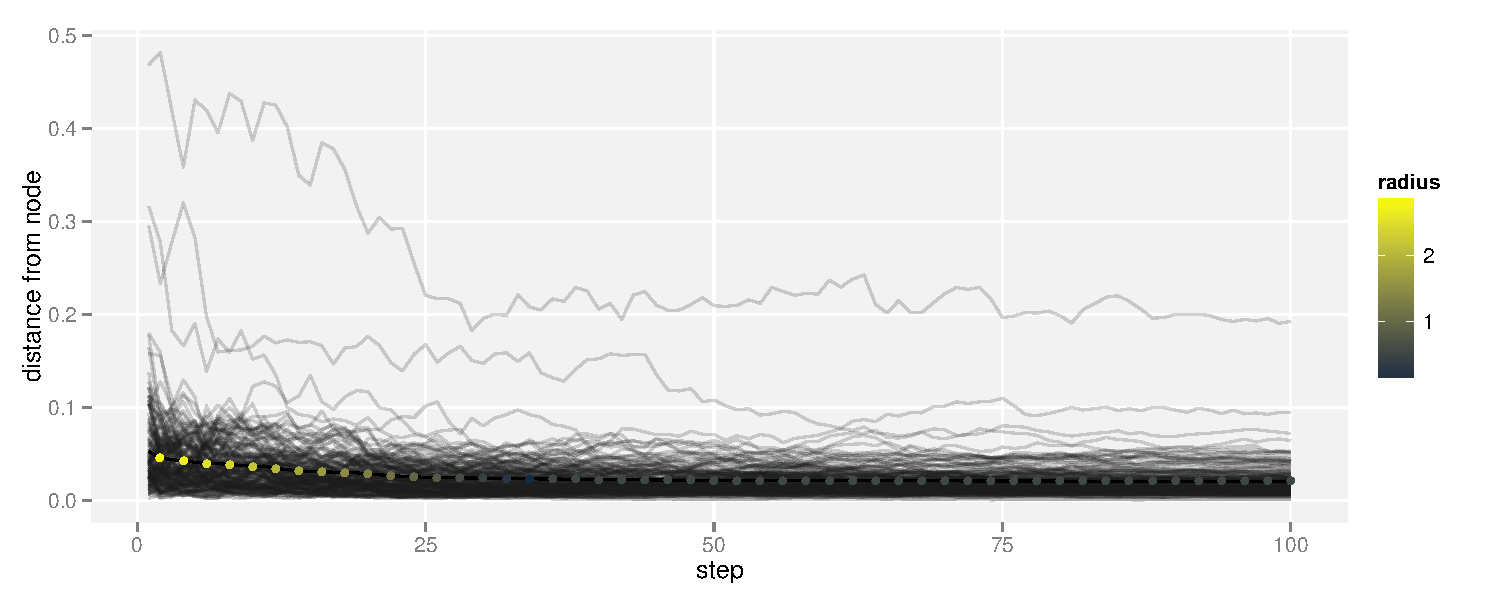
\includegraphics[width=5in]{som-dist}
  \caption{(Top) Time series of mean distance from point to corresponding node, over time.  (Bottom) Distance to corresponding node for each individual point.  Note the difference in scale!  Mean points are colored by radius.  Alpha is not displayed, but deceases linearly from 0.05 to 0.}
  \label{fig:som-dist}
\end{figure}

To see how the model changes over time, Figure~\ref{fig:iteration} displays the model in the data space for four selected iterations.  A movie showing more iterations, more views of the model, and interaction between the model and model summaries is available at \url{http://vimeo.com/823541}.  It's interesting to note that the green and orange clusters are close in the data space, but distant in the model space.  We could improve our {\sc som} model by joining the two ends.  We also might have expected that the middle of the net would go through the green group, not the purple group, but this is likely a function of the initialization. With increasing iterations the model expands out and is closer to joining the two ends, but also becomes more twisted. It may be too many iterations.

\begin{figure}[htb]
  \centering
    \includegraphics[width=1.5in]{step-001.pdf}
    \includegraphics[width=1.5in]{step-005.pdf}
    \includegraphics[width=1.5in]{step-025.pdf}
    \includegraphics[width=1.5in]{step-100.pdf}
  \caption{Iterations 1, 5, 25 and 100 shown in the same tour projection.  After five iterations the model seems to run through the center of clusters fairly well, and continues to change some over the next 99 iterations.  The net  extracts a 1d path between the 3 groups, and then expands further. }
  \label{fig:iteration}
\end{figure}

When we first used this package, it was not possible to break up the iterations into single steps, because there was not sufficient control over the changes to $r$ and $\alpha$.   After asking the package author to give access to the iterations, this visualization revealed some problems with the implementation of the {\sc som}.   The m-in-ds visualization also revealed that the nets were twisted and tangled up.  The author has since fixed these initial bugs.

\section{Pulling it all together: Visualizing neural networks}
\label{sec:nnet}

This case study pulls together all three themes of the paper to develop visualizations that investigate the fit of single-hidden-layer neural networks, as implemented by the {\tt nnet} package \citep{mass}.  Much like self organizing maps, neural networks are often treated as black boxes, and are used purely for prediction and not to give insight into the data. We want to dig deeper, and explore how they work, how well they work, and what we need to do to get the best performance.  This longer case study is broken up into three parts:

\begin{itemize} \itemsep 0in
  \item  In Section~\ref{sub:minds} we  develop a visualization of the output of the neural network in the data space, based on ideas from the classification section.

  \item The definition of neural networks reveals that they are an ensemble model, composed of multiple logistic regressions. In Section~\ref{sub:ensemble} this insight  leads us to develop a visualization that shows what the internal sub-models are doing.

  \item The parameters of a neural network are estimated with a numerical method and often get stuck in local optima.  Section~\ref{sub:starts} explores why this happens and how to ensure we get a good fit, by visualizing many random starts and the process of iteration.

\end{itemize}

We illustrate this section with a simple two class, two dimension, classification problem, shown in Figure~\ref{fig:nnet-test}. The two classes can be completely separated by a non-linear boundary, easily drawn in by hand: the human neural network can easily solve this problem! Even a simple linear classifier does well on this dataset, correctly classifying 92\% of the points. This is a simple problem but it reveals many interesting features of neural networks.

\begin{figure}[htbp]
  \centering
    \includegraphics[width=0.45\textwidth]{nnet-test}
  \caption{Simple two class, two dimension, classification problem.  The classes can be completely separated by an easily seen non-linear boundary.}
  \label{fig:nnet-test}
\end{figure}

\subsection{Model in data space}
\label{sub:minds}

Assume we have been given a fitted neural network model.  How can we visualize it?  The basic output from the model is a prediction surface for each class, giving the probability that a new observation at $(x, y)$ belongs to that class.  In the two class case, we only need to look at one of these surfaces, as the two probabilities must sum up to 1.  To visualize this surface, we have two basic options, shown in Figure~\ref{fig:nnet-best}. We could draw an image plot showing the probability at each location, or summarize the shape with a few contour lines, here at 10\%, 25\%, 50\%, 75\% and 90\%.  The 50\% boundary determines whether a new observation is classified as class A or B.  Both displays show that the boundary does what we intuitively expect, and that the classification boundary is very sharp; this classifier is quite certain which class a new observation should be given.

\begin{figure}[htbp]
  \centering
    \includegraphics[height=2.5in]{nnet-best-fill}
    \includegraphics[height=2.5in]{nnet-best-contour}
  \caption{visualizing the classification surface.  (Left) An image plot, showing probability that a new observation belongs to class B, and (right) a contour plot showing five iso-probability contour lines (10\%, 25\%, 50\%, 75\%, 90\%).  This classifier perfectly distinguishes the two classes, and is very sharp.}
  \label{fig:nnet-best}
\end{figure}

\subsection{Looking at multiple models: ensemble}
\label{sub:ensemble}

A single-hidden-layer neural network is composed of a set of sub-models, logistic regressions, whose outputs are combined using another logistic regression.  In the terminology of neural networks, the sub-models are hidden nodes, and the number of these nodes is the single most important tuning parameter.  The hope is that these sub-models  identify important lower-level features which can then be combined to reveal important high-level features, much in the same way that biological neural networks (brains) work.

To be more precise, the probability that unit $y$ with values $x_{1}, ..., x_{p}$ belongs to class $j$ is

\[
P(y \in \textrm{class}_j | x_{1}, ..., x_{p}) = k \cdot \phi ( \alpha + \sum_{h=1}^s w_{hj} \phi (\alpha_h + \sum_{i=1}^p w_{ih} x_i ))
\]

\noindent where $s$ is the number of hidden nodes, $p$ is the number of explanatory variables, and $k$ is a normalization constant which ensures that the probabilities for all classes add up to one.  The function $\phi$ can be anything but is usually taken to be the logit for classification problems.

So far we have just looked at the overall output of the model, but we can also dig in and see what the hidden nodes are doing.  Each internal node is a logistic regression, so we can visualize it the same way as the overall output, except that now we need to display the output for each node.  Since there only a few models, we can display each side-by-side, or  superimpose the 50\% contour line on a single plot.  Note that output from the internal nodes does not map directly to a prediction class, but is used by the final logistic regression to generate classification probabilities. For our model, these displays are shown in Figure~\ref{fig:nnet-internal}.  Each internal node has a sharp boundary which identifies part of the piece-wise linear path that separates the groups.

\begin{figure}[htbp]
  \centering
    \includegraphics[width=6in]{nnet-hidden-fill}
    \includegraphics[width=0.45\textwidth]{nnet-hidden-contour}
  \caption{visualization of the hidden nodes of a neural network.  (Top) The probability surfaces for the hidden nodes are displayed side-by-side.  (Bottom) The 50\% probability contours from the nodes are overlaid on a single plot.  We see how each node identifies one linear break producing the final classification boundary shown in Figure~\ref{fig:nnet-best}.}
  \label{fig:nnet-internal}
\end{figure}

This plot hints at some of the difficulties faced when estimating the model parameters.  The parameters are over-specified, as we can swap any two hidden nodes, or flip the direction of logistic regressions along the boundary lines, and still get the same overall model.

\subsection{Looking at multiple models: random starts}
\label{sub:starts}

The parameters of the neural network are estimated by numerical optimization.  Neural networks often converge to local optima and it is customary to try multiple random starts to find the global optima.  For our dataset, we  try 200 random starts each for neural networks with two, three and four hidden nodes.  This gives a total of 600 neural networks fit to the data.   Figure~\ref{fig:nnet-many} summarizes the results. There is a striking variation in the ability of the neural network to correctly separate the two classes, with prediction accuracy ranging from 80\% to 100\%.  Most of the networks correctly classify 92\% of the points, no better than a linear boundary.  Only one network classifies the training data perfectly!  Interestingly, increasing the number of nodes does not affect the predictive ability of the majority of the networks, but, surprisingly, does increase the number of very good and very bad models.

\begin{figure}[htbp]
  \centering
    \includegraphics[width=4in]{nnet-value-accuracy}
    \includegraphics[width=4in]{nnet-accuracy}
  \caption{Summary of 600 neural networks with two, three and four hidden nodes.  (Top) Scatterplot of prediction accuracy vs internal criterion.  (Bottom) Histograms of prediction accuracy.  Most networks achieve an accuracy of 92\%, with just a few that do much better or much worse.}
  \label{fig:nnet-many}
\end{figure}

Figure~\ref{fig:nnet-all4} shows the classification boundaries of all 600 neural networks roughly broken down by model quality (sub-linear, linear, super-linear, excellent).  There is a lot of overplotting, but we can see that many of the networks have a linear classification boundary, some seem to get one of the gaps, but not both, and a number of the four-node models capture the essence of the boundary, even if they are not completely correct.

% This graphic would be considerably enhanced with interaction.  We be able to select boundaries and see other information about the model: prediction accuracy, internal criterion value, values of tuning parameters.  Or we could link in the opposite direction, selecting interesting models based on their summary statistics and then seeing those models embedded in the data space.

\begin{figure}[htbp]
  \centering
    \includegraphics[width=6.5in]{nnet-all}
  \caption{Classification boundaries from all 600 neural networks, subset by model accuracy and described based on the boundary form as sub-linear, linear, super-linear, or excellent.  Sub-linear models have accuracy in $[0\%, 91.5\%]$, linear in $[91.5\%, 92.5\%]$, super-linear in $[92.5\%, 98\%]$, and excellent in $[98\%, 100\%]$. Most of the boundaries are linear, a few get one of the bumps, and quite a few of the four node networks get the overall form right, even if they are not perfectly accurate.}
  \label{fig:nnet-all4}
\end{figure}

We can also use this same idea to explore the process of model fitting, treating each iteration as a model in its own right. The video at \url{http://www.vimeo.com/767832} shows the changes in the hidden nodes as the algorithm proceeds.  An alternative approach is to display the iterations simultaneously by only showing the 50\% boundary, as in Figure~\ref{fig:nnet-iteration}.  We can see the boundaries move rapidly at first, and then appear to stabilize.

\begin{figure}[htbp]
  \centering
    \includegraphics[width=6in]{nnet-iteration}
  \caption{How the 50\% probability line for each node changes with time.  100 runs with 5 iterations between each.  Nodes start similarly, move rapidly in the first few iterations, then slow down, converging to surfaces that are quite different.  Animated version available at \url{http://www.vimeo.com/767832}.}
  \label{fig:nnet-iteration}
\end{figure}

\subsection{Real data}

Even though we have used a very simple example we have still discovered many interesting features of the neural network algorithm.  In real life the neural network is considerably more complicated due to more data points, more internal nodes, and more possible classes.  However, we can continue to use the same ideas, with a few tweaks:

\begin{itemize} \itemsep 0in
  \item If there are more than two classes, we can no longer summarize the model with a single probability surface, but we  need one for each class.  When computing classification boundaries we  need to use the advantage statistic developed in Section~\ref{sub:classifly}.

  \item If there are more than two input variables, we  need to use high-dimensional tools to visualize the classification surface such as described in Section~\ref{sub:classifly}.

  \item More data points should not affect our choice of visualizations, but it  makes the neural networks slower to fit.  This may affect our ability to try the many possible random starts necessary to find a good fit.

\end{itemize}

\section{Conclusion}
\label{sec:conclusion}

We have presented three important strategies for visualizing models: visualize the model in data space, collections are more informative than singletons and explore the process of model fitting.  These were illustrated with many case studies that developed informative visualizations using the strategies outlined in the paper.  Many of these techniques have grown out of our work with {\tt rggobi} \citep{rggobi}, an R package which connects the statistical programming environment of R \citep{r} with the interactive and dynamic graphics of GGobi  \citep{swayne:2003}. This paper ties together the ideas underlying three R packages that use {\tt rggobi}: {\tt classifly} \citep{classifly}, {\tt clusterfly} \citep{clusterfly}, and {\tt meifly} \citep{meifly}.  The tight connection between R and GGobi facilitated the development of all of the examples, and has resulted in the development of R packages that one can easily download and try out.

To make these tools useful in practical model building we need to improve our ability to visualize high-d data and surfaces.  We have the basic tools, but as the number of dimensions increases, the number of potential views becomes overwhelming.  How can we provide support for finding revealing views, while maintaining the ability of the analyst to look for the unexpected?  We have touched on projection pursuit for finding interesting views of the data, and we expect developing descriptive statistics that summarize both the model and data to be a fruitful approach.  The challenge is, as always, developing good summaries, but our graphical tools can help us develop these for low-d data for application to high-d data.

We also need better tools to visualize high-d surfaces.  In this paper we have gone to considerable lengths to approximate high-dimensional surfaces with a dense set of points.  Development of better sampling methods would be useful, but the development of higher dimensional drawing primitives is more of a priority.   GGobi currently provides 0d (points) and 1d (lines) primitives, can we supplement these with 2D primitives (triangles?) as well?  The development of adaptive contouring algorithms for high-d would also be useful.

The case studies in this paper are just a beginning and we hope that others pick up these ideas to develop visualizations for more models in a wider array of statistical and graphical environments.

\section{Acknowledgements}

This material is based upon work supported by the National Science Foundation under Grant No. 0706949.


\bibliographystyle{abbrvnat}
% bibtool -x model-vis.aux -o references.bib
\bibliography{references}

\end{document}
